% -*- coding: utf-8 -*-
%%
%%  本模板可以使用以下两种方式编译:
%%     1. PDFLaTeX
%%     2. XeLaTeX [推荐]
%%  注意:
%%    1. 在改变编译方式前应先删除 *.toc 和 *.aux 文件,
%%       因为不同编译方式产生的辅助文件格式可能并不相同。
%\documentclass[nocover]{cumcmart}%%%切换到无封面的版本,有些区域不允许前面的承诺页用pdf格式,可以用此去掉。
% 已经修改了模版,默认不要封面
\documentclass[12pt]{cumcmart}   %调用模板文件.cls
\usepackage{comment}       %调用注释宏包
\usepackage{booktabs}      %使用三线表
\usepackage[section]{placeins}  %让浮动体无法超过section
\usepackage{array}
\usepackage{graphicx}      %使用缩放盒子
\usepackage{multirow }
\usepackage{float}
\usepackage[super,square, sort,compress]{natbib}%%%%%%%%%%%%%参考文献格式设置
\usepackage{ tabularx}



\usepackage{listings} %调用高质量展示代码的宏包
\lstset{breaklines}%自动将长的代码行换行排版
\lstset{extendedchars=true}

\definecolor{grey}{rgb}{0.8,0.8,0.8}
\definecolor{darkgreen}{rgb}{0,0.3,0}
\definecolor{darkblue}{rgb}{0,0,0.3}  
%\def\lstbasicfont{\rmfamily\normalsize }
\def\lstbasicfont{\setmainfont{Courier New} \normalsize   }
\lstset{%
	% numbers=left,   
	% numberstyle=\small,%
	showstringspaces=false,
	showspaces=false,%
	tabsize=4,%
	frame=lines,%
	basicstyle={\footnotesize\lstbasicfont},%
	keywordstyle=\color{darkblue}\textbf,%
%    keywordstyle=\color{blue!70}
	identifierstyle=,%
	commentstyle=\color{darkgreen},%\itshape,%
%	stringstyle=\color{black}%
	stringstyle=\rmfamily\slshape\color[RGB]{128,0,0},   % 设置字符串格式
}
\lstloadlanguages{C,C++,Java,Matlab,Mathematica,Python,R}


\begin{document}
\renewcommand{\baselinestretch}{1.3}\normalsize  % 调整行距
\zihao{-4}

\title{基于三角函数拟合与遗传算法的太阳影子定位分析}


\maketitle
\begin{cnabstract}%此处没有采用sbstract命名,是为了将来如果要加入英文摘要时扩展的方便
确定视频的拍摄地点和拍摄日期是视频数据分析的重要方面,太阳影子定位技术就是通过分析视频中物体的太阳影子变化,确定视频拍摄的地点和日期的一种方法。依据影子长度进行地理定位的精度提高以及提升对视频中进行图像处理的精度成为太阳影子定位技术的两大核心任务。

针对问题一,本文基于地理、天文学知识给出了计算影子长度的数学模型。经分析,太阳影子长度受日期、经纬度、杆长、北京时间的影响。其中,年份对太阳影子长度的影响可以忽略;积日对影长的影响呈夏短冬长(南半球则相反);相等的影长在经纬度上呈环状分布,并且纬度越高,影子越长。随着纬度的增加,影长增加的越来越快;最后求出的影子长度变化曲线在日出和日落时均存在影长突变的情况。

针对问题二,基于问题一的影长函数结构,本文自定义了一个能够高度近似原影长函数的三角拟合函数,通过拟合求解出当地经度为$109.6575^\circ$并由拟合出的系数给出了杆长与纬度的预测值2米、$22.5^\circ$,相当于预测了一个地理位置。然后基于最小二乘法给出了适应度函数并使用遗传算法进行求解。遗传算法搜索出两个较优解$18.41^\circ,-0.13^\circ$。可见其中一个与预测效果相差不大。附件一提供的数据为4月18日,太阳直射北半球。可见搜索出的两个最优解基本关于直射点对称。故而推测最可能的地点为:海南岛三亚和西加里曼丹。


针对问题三,相当于在问题二的基础上增加了积日这个变量。为了保证自定义的拟合函数拟合效果,针对积日的变动对拟合函数进行了改进并求解出经度为$79.6857^\circ$。随后采用与问题二相同的方法求解。对于附件二,遗传算法搜索结果中纬度为$39.5341^\circ$、杆长为2.0403米、积日为203天的适应度函数最低且与预测值$39.8433^\circ$、1.99099米、141天十分相近。故而推测最可能位于新疆西部地区,时属4月份或7月份;同理可推知附件三中最可能位于湖南张家界地区,时属10月份。

针对问题四,我们先对视频按一分钟每帧截取了41张图片,通过透视变换,将截取的原始图片的影子投影变换为光线垂直于地面的正投影。然后对变换后图片进行一系列处理,通过引入水平辅助线,计算出真实影子长度。结合问题二、三,有日期时视频拍摄地的可能地点位于桂林而没有日期时视频拍摄地的可能位于陕西并时属6、7月份。最后对模型求解过程可能存在的误差以及对经度变化对求解结果的影响进行了分析。



\cnkeywords{太阳影子定位\quad 三角函数拟合\quad 遗传算法\quad 透视变换}
\end{cnabstract}

\newpage
%\tableofcontents%增加目录,要不要都可以。不想要的话,就在本行前加“%”(英文的百分号)
 \setcounter{page}{1}
\pagestyle{fancy} 
\section{问题重述}
\subsection{问题背景}
根据美国能源信息署 EIA 发布的国际能源展望,世界能源市场消耗量 2005 年到 2030年预计增加50\%,CO2的排放量将由 281 亿吨增至 423 亿吨,而 CO2的排放中,有四分之一来自于汽车尾气。目前,世界各国的交通工具主要以燃油为主,且燃油汽车数量还在不断的快速增长之中,燃油汽车在消耗大量能源的前提下,还造成了严重的环境问题。

 新能源汽车的研发与应用对日益紧张的能源形势和环境问题的巨大缓解作用已经引起了世界多数国家的重视,被认为是 21 世纪汽车工业改造和发展的主要方向。2015 年 5 月,我国在国务院正式印发的《中国制造 2025》中,明确定义节能与新能源汽车为 10 大重点领域之一。工信部部长苗圩在接受央视专访时透露,国家确定了节能与新能源汽车 2019 年要占到 8\%,2020 年要占到 10\%的奋斗目标,取消燃油车的时间表正在研究之中。荷兰、挪威、法国等欧洲国家更是已经发布了燃油汽车禁售时间表。 
 
 电动汽车作为新能源汽车的代表,近年来发展迅速,据 EV Sales公布的数据显示,2017 年全年全球电动车销量超过 1,223,000 辆,对比 2016 年增长 58\%,进而促使全球电动汽车销量在全球汽车销量当中的占比超过 1\%。作为电动汽车重要的服务设施,充电站的位置、类型、数量等对电动汽车未来的发展起着至关重要的作用,对消费者购买电动汽车意愿有着重大影响。 
 
 


\subsection{问题提出}
假设我国的内部、外部政策环境、经济增长速度、主要基础设施等保持不变,充电站仍为两种类型,即快速充电类型(超级充电或直流充电)和普通充电类型(目的地充电或交流充电),完成下述问题: 

\begin{enumerate}
	\item 建立数学模型,探讨电动车数量与充电站数目、类型以及位置之间的关系规律。
	\item 应用你所建立的数学模型针对某个国家或某个地区进行计算,通过与该地区实际的充电站数目、类型以及位置进行对比,对模型进行验证、评价。(提示:充电站相关数据可以参考 tesla 公司网站,国内大城市,例如北京,亦有充电站位置分布网站或(APP) 
	\item 以陕西省为例,假设至 2050 年,陕西省内所有出租车和私家车全部转换为电动车,试计算所需的充电站数量、类型,位置,以及为建设这些充电站所投入的资金数量。 
\end{enumerate}





\newpage

\section{问题分析}
确定视频的拍摄地点和拍摄日期是视频数据分析的重要方面,而太阳影子定位技术就是通过分析视频中物体的太阳影子变化,确定视频拍摄的地点和日期的一种方法。影子长度的变化需要以地理学、天文学为基础进行推导。当影子长度确定后,要实现地理定位便需要进行搜索。于此同时,对已知数据的拟合效果直接决定了搜索的效果
\subsection{问题一的分析}
问题一关键在与建立地理、天文学变量之间的关系。但是对一些天文学变量往往很难计算其准确值。因此可以选取一些误差非常小的近似公式作为代替推导出影子长度与经纬度、积日、杆长、时间之间的关系。最后进行单一变量分析并给出指定条件下的影子长度变化曲线。
\subsection{问题二的分析}
问题二关键在于给出可能性高的衡量标准。为了提高搜索的精度,可以先用拟合的方法求出经度。由于问题一中给出了函数结构,故可以自定义一个拟合函数,使其不仅能求出经度,也能提供纬度、杆长的预测值。然后可以基于最小二乘法的思想,利用遗传算法中每一代的变量值计算出附件一中每一时刻对应的函数值,并与提供的数值作差并平方,衡量每一个样本点的误差。将21个样本的误差和作为适应度函数进行搜索求解即可。
\subsection{问题三的分析}
问题三是在问题二的基础上增加了积日这一个变量,但是却给搜索带来了精度上的挑战。为使得拟合函数能够近似表征原有函数,需要对问题二中的拟合函数进行修改。进而采用三个变量的遗传算法对问题三进行求解。
\subsection{问题四的分析}
问题四的关键在于如何将视频中影子的中心投影转换为平行投影,从而计算出影子的实际长度。所以首先需要对视频图像进行截取,然后对图像进行透视变换,转化为平行投影之后,经过对图像的一系列处理,采用添加辅助线的方式,得出影子的实际长度。再结合问题二与问题三的模型,分别给出有无日期情况下的可能求解结果。

\newpage

\section{模型假设}
\begin{center}
\begin{enumerate}
\item 假设地球是一个正球体
\item 假设太阳光为平行光且大气对太阳光的折射可以忽略
\item 假设地面可以看成一个水平面且被测直杆垂直于地面
\end{enumerate}
\end{center}

\section{符号说明}
\begin{center}
	\begin{tabular}{cc}
		\hline
		\makebox[0.3\textwidth][c]{符号}	&  \makebox[0.4\textwidth][c]{意义} \\ \hline
		$L$ & 直杆长度\\ \hline
       $l$  &  影子长度  \\ \hline
	  $\delta$  & 太阳赤纬角  \\ \hline
	 $\alpha$     & 太阳高度角  \\ \hline
	 	 $\psi$     & 纬度  \\ \hline
	 	 $\phi$     & 经度  \\ \hline
	 	 	 $\omega$     & 时角  \\ \hline
	 	 	 	 $N$     & 积日  \\ \hline
	 	 	 	 $t$     & 当地北京时间  \\ \hline
	 	 	 	 $T_c$     & 地方时  \\ \hline
	 	 	 
	\end{tabular}
\end{center}


\section{模型的建立与求解}

\subsection{问题一影子长度变化模型的建立与分析}

\subsubsection{影子长度变化模型的建立}
基于地理学与天文学知识,本文给出了以经纬度、时间、杆长为自变量的影子长度变化的数学模型。

在已知杆长$L$的前提之下,只需要一个太阳高度角$\alpha$便可以求出影子长度。具体物理情形如图~\ref{tan}~。太阳高度角是指太阳光的入射方向和地平面之间的夹角,专业上讲太阳高度角是指某地太阳光线与通过该地与地心相连的地表切面的夹角。
\begin{figure}[H]
	\centering
	
\includegraphics[scale=0.3]{images/tan.png}
	\caption{太阳高度角}
	\label{tan}
\end{figure}
由图~\ref{tan}~易知有
\begin{equation}
tan \alpha=\frac{L}{l}
\end{equation}
其中$L$为杆长,$l$为影子长度,$\alpha$为太阳高度角。查阅相关资料,给出以下太阳高度角计算方法:

设$\psi$为纬度,$\phi$为经度,$\omega$为时角,$\delta$为太阳赤纬角。其几何意义如图~\ref{xiangguanjiao}~所示($\omega_0$表示日出时角)。
\begin{equation}
sin \alpha=sin \psi sin\delta +cos \omega cos \psi cos \delta
\label{qiumian}
\end{equation}
\begin{figure}[h]
	\centering
	
\includegraphics[scale=0.4]{images/diqiu.png}
	\caption{太阳相关角度}
	\label{xiangguanjiao}
\end{figure}
利用球面三角函数公式,可以得到


下面给出太阳赤纬角$\delta$和太阳时角$\omega$的计算方法:
\begin{enumerate}
	\item 太阳赤纬角亦称黄赤交角(又名:黄道交角)是地球公转轨道面(黄道面)与赤道面(天赤道面)的交角,也称为黄赤大距。目前地球的太阳赤纬角为约为$23^\circ 26'$。查阅资料 \cite{Wu2017A} 知其计算公式满足以下公式:
	\begin{align}
	\delta=&0.3723+23.2567sin\theta+0.1149sin2\theta-0.1712sin3\theta\\
	&-0.758cos\theta+0.3656cos2\theta+0.0201cos3\theta \notag  \\
		\theta=&\frac{2\pi (N-N_0 )}{365.2422} \\
		N_0=&79.6764+0.2422 \times(year-1985)-[\frac{year-1985}{4}]
	\end{align}
	其中,$\theta$为日角(单位:度),用于衡量地球的公转过程。$N$为积日,其值等于测试影长的日期到1月1日的时间,平年时积日的最大值为365天,闰年最大值为366天。$\Delta N$表示积日修正日,$N_0$实际上是对平年、闰年的一种修正;year 为年份,问题一中为2015年,从而$N_0=79.9424$;$[\quad]$为向下取整运算,相当于MATLAB中的$floor$,如$[3.1]=3$;从上式中可以看出太阳赤纬角仅与和积日、年份有关。
	
	
	\item 一个天体的时角表示该天体是否通过了当地的子午圈(中天)。其数值则表示了该天体与当地子午圈的角距离,并借用时间的单位,可以用小时来计量(1HA = 15度)。例如,一个天体的时角是2.5HA,就表示他已经在2.5个小时之前通过当地的子午圈,并且在当地子午圈的西方37.5度的距离上。负数则表示在多少小时之后将通过当地的子午圈。从文献中可查到其表达式(单位:rad):
	\begin{align}
\omega=&\pi(\frac{T_c-12}{12})    \label{shijiao} \\
	  T_c=&\frac{\phi-120^\circ}{15}+t_c\\
	  t_{c}=&t+\frac{\Delta t}{60}\\
	  \Delta t=&0.0028-1.9857sin\theta+9.9059sin2\theta-\\
	  &7.0924cos\theta-0.6822cos2\theta  \notag
	\end{align}
	上式中,$T_c$为当地地方时,$t_{c}$为真太阳时。并且:真太阳时=平太阳时+真平太阳时差:	$t_{c}=t+\Delta t$,其中$\Delta t$为平太阳时(北京时间$t$)和真太阳时时差(只与积日有关)。$\Delta t$(单位:分)为平太阳时(北京时间$t$)和真太阳时时差。从上式中可以看出时角与经度、真太阳时(修正的北京时间)有关。
	\item 影子长度和杆长显然呈正比关系(其他变量保持一定时),此处不再详细讨论。
\end{enumerate}

\makebox{}

联立以上公式,可以得出影子长度$l$的总表达式:($\alpha \in (0,\frac{\pi}{2})$)
\begin{align}
l=&\frac{L\sqrt{1-(sin\alpha)^2}}{sin\alpha} \label{lalpha} \\
sin \alpha=&sin \psi sin\delta +cos \omega cos \psi cos \delta \notag \\
\omega=&\pi(\frac{T_c}{12}-1) \notag \\
\delta=&\frac{469\pi sin(\frac{2\pi(N+284)}{365})}{3600}  \label{deta}
\end{align}

\subsubsection{影子长度变化的因素分析}
由上述分析可知太阳影子长度与日期、经纬度、杆长、当天北京时间有关。而日期又包括年份与积日两个部分。下面分别考虑这些因素对太阳影子长度的影响:

\begin{enumerate}
	\item 年份对太阳影子长度的影响:画出北京市1988到2016年之间,10月22日上午9时整的影子长度变化曲线如图~\ref{nianfen}~所示。图中有明显的周期与分层现象,这种现象归结于闰年、平年的周期变换,故而图像中层次与周期均为4。我们知道,地球的公转过程是有误差的,天文学中也有很多的矫正公式,而我们上述模型中使用的也仅是近似公式,故而出现了影子长度每四年均上升一定长度的现象。但是由于这种增长速度相对来说及其缓慢,这些公式往往可以用于平时的计算过程中。由图~\ref{nianfen}~可以计算,在这29年内,最大的影子长度平均年变化率为\[p=\frac{6.72-6.70}{6.70\times 28}\times 100\%=0.016\%\]可见由年份造成的误差几乎可以忽略,因此,本文在后续讨论中均不考虑年份的影响。
	\begin{figure}[h]
		\centering
		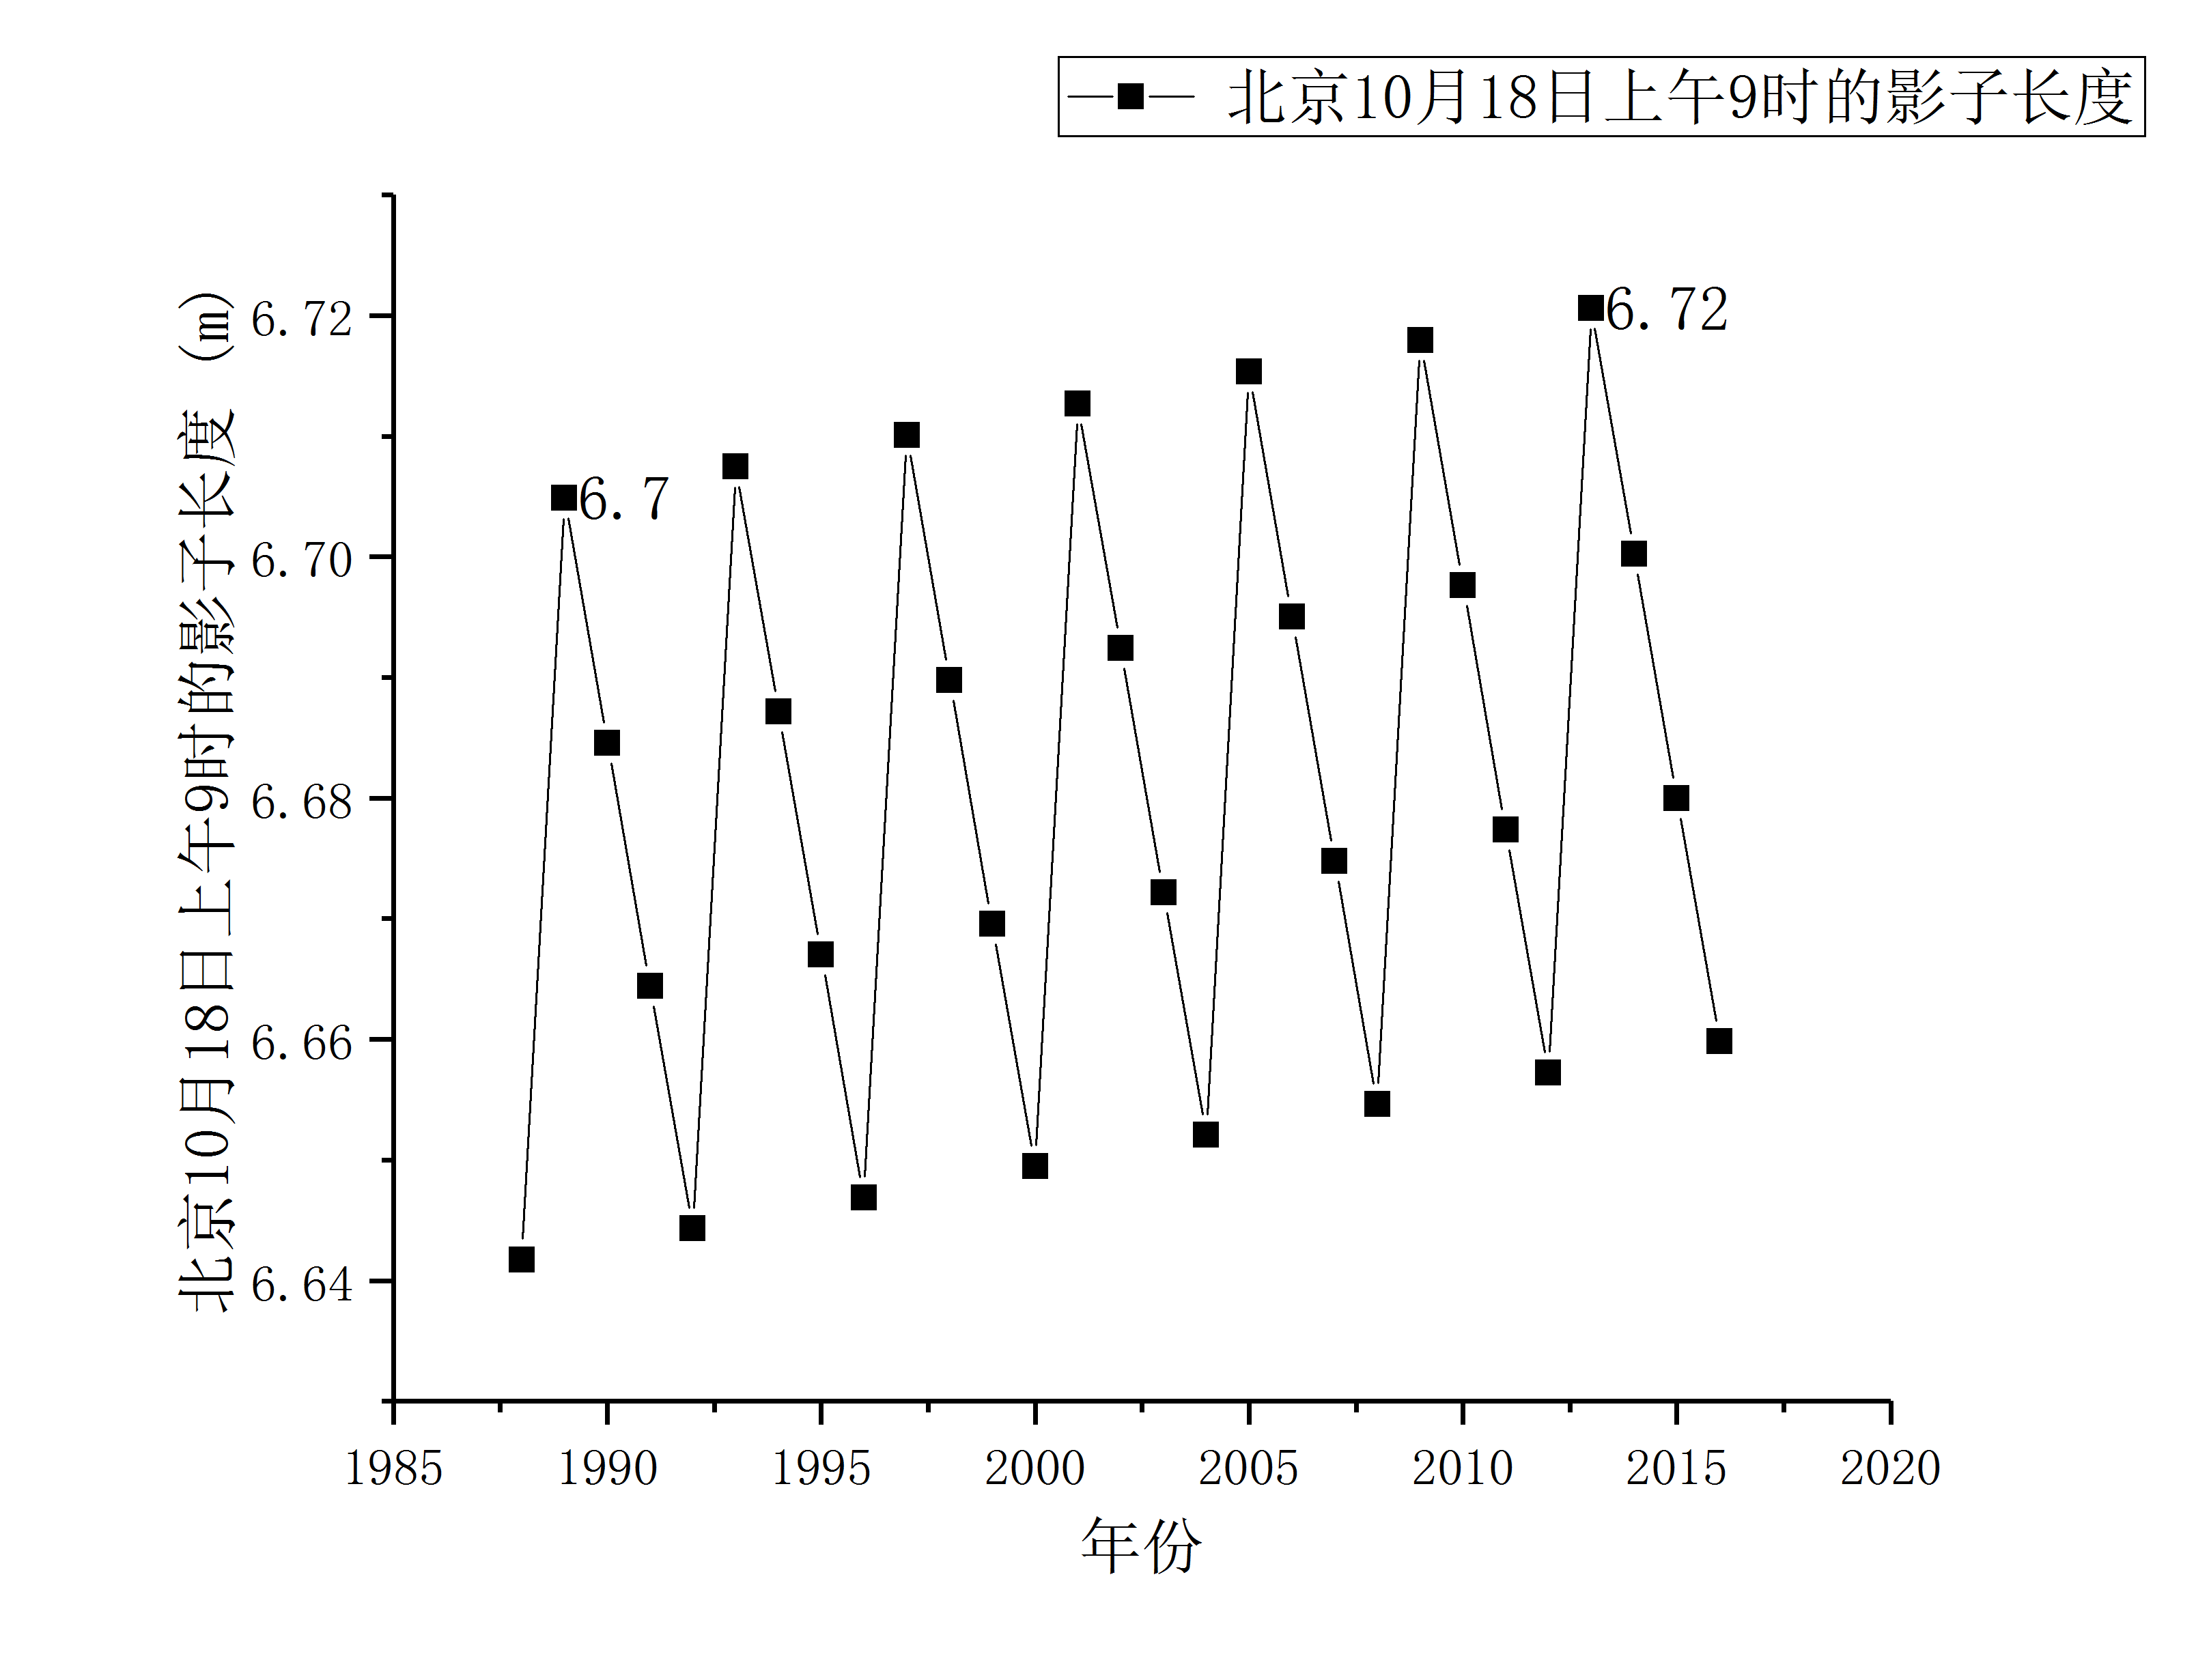
\includegraphics[scale=0.4]{images/nianfen.png}
		\caption{年份对太阳影子长度的影响}
		\label{nianfen}
	\end{figure}
	\item 积日对太阳影子长度的影响:画出2015年北京时间9点全年的太阳影子长度变化图如~\ref{nianjiri}~所示。图中可以明显反映出北京四季的变化。夏季影子短,影子长度处于图中低谷阶段;冬季影子长,影子长度处于图中峰值阶段。
	      
	    \begin{figure}[H]
	  	\centering
	  	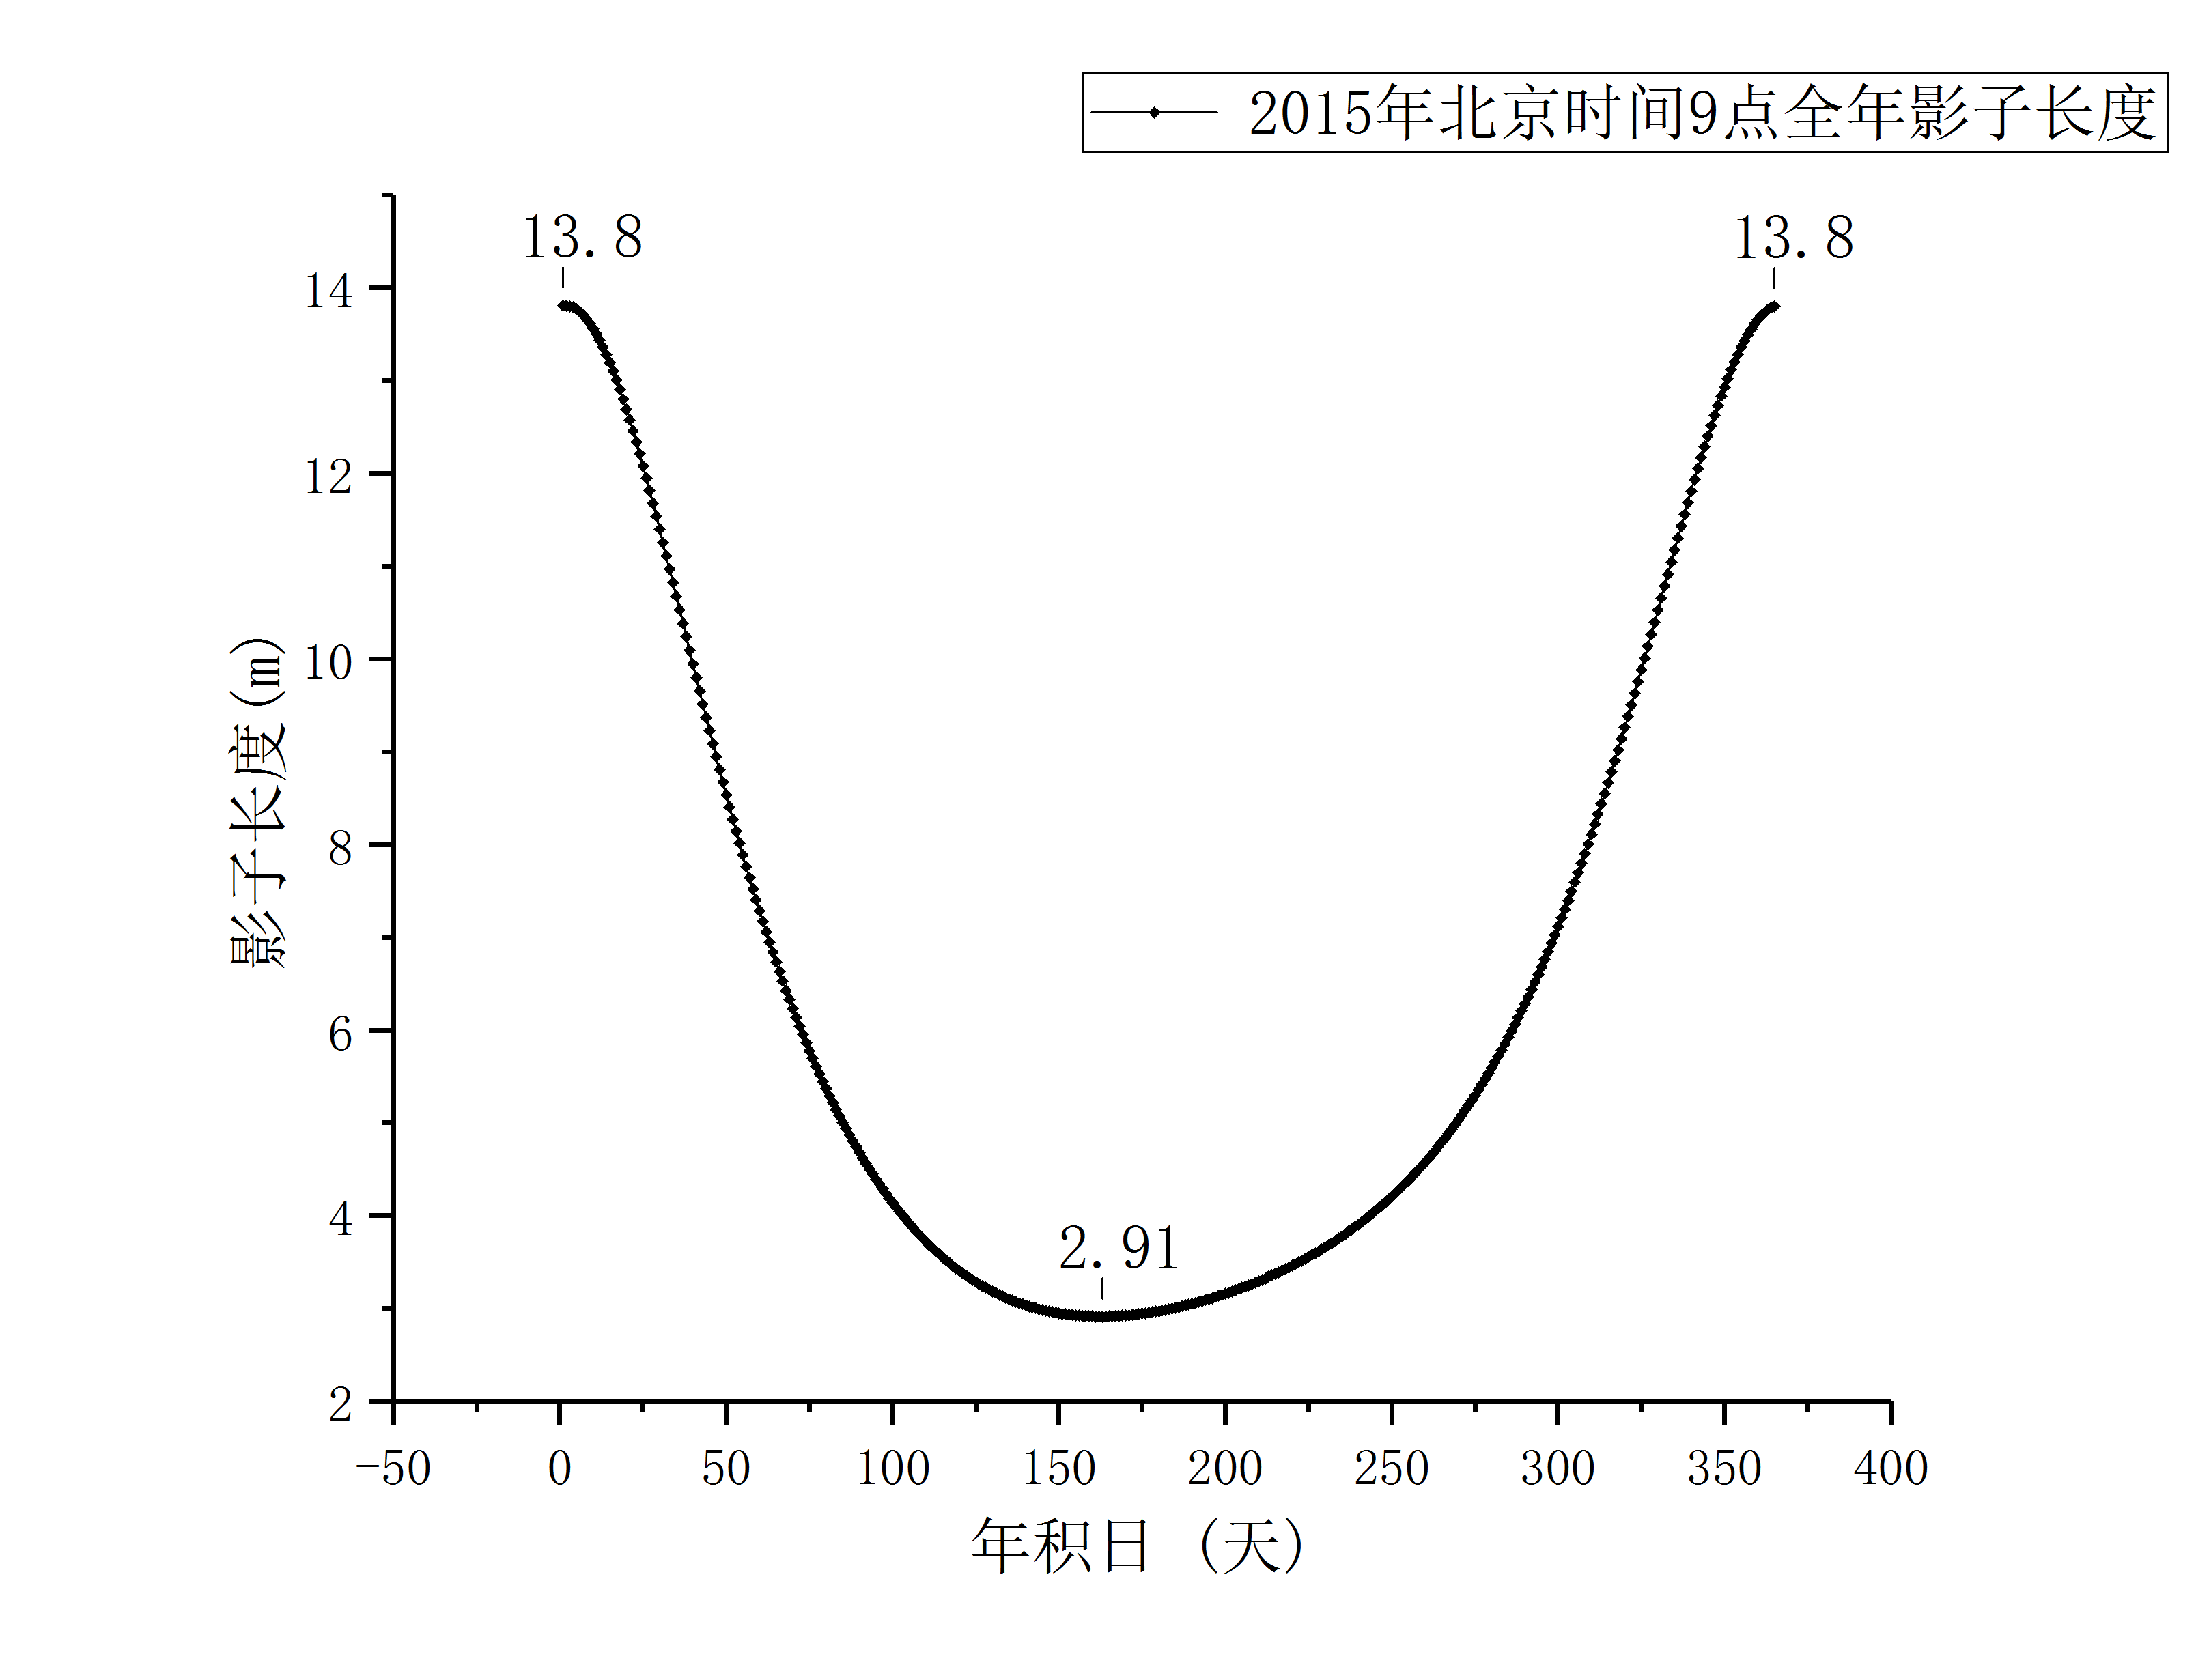
\includegraphics[scale=0.4]{images/nianjiri.png}
	  	  \caption{积日对太阳影子长度的影响}
	  	\label{nianjiri}
	  \end{figure}    
  
  \item  经纬度对太阳影子长度的影响:经初步验算,2015年10月22日北京时间上午九点太阳应该直射南半球且影子长度为零的点应该在东经$120^\circ$以东。故而本文选取南纬$[-30^\circ,-10^\circ]$,东经$[150^\circ,170^\circ]$为$XY$面绘制出影子长度关于经纬度的三维图像如图~\ref{jingwei}~所示。图中曲面上的黑色弧线为等高线,可见以太阳直射点为中心,太阳向四周辐射的相等影长呈环状分布(同一时间,相同杆长)。观察东经$150^\circ$可以发现在太阳直射点以南,纬度越高,影子越长。而且,随着纬度的增加影子长度增加的越来越快。对经度也有类似的结论。
  	       
  	      \begin{figure}[H]
  	     	\centering
  	     	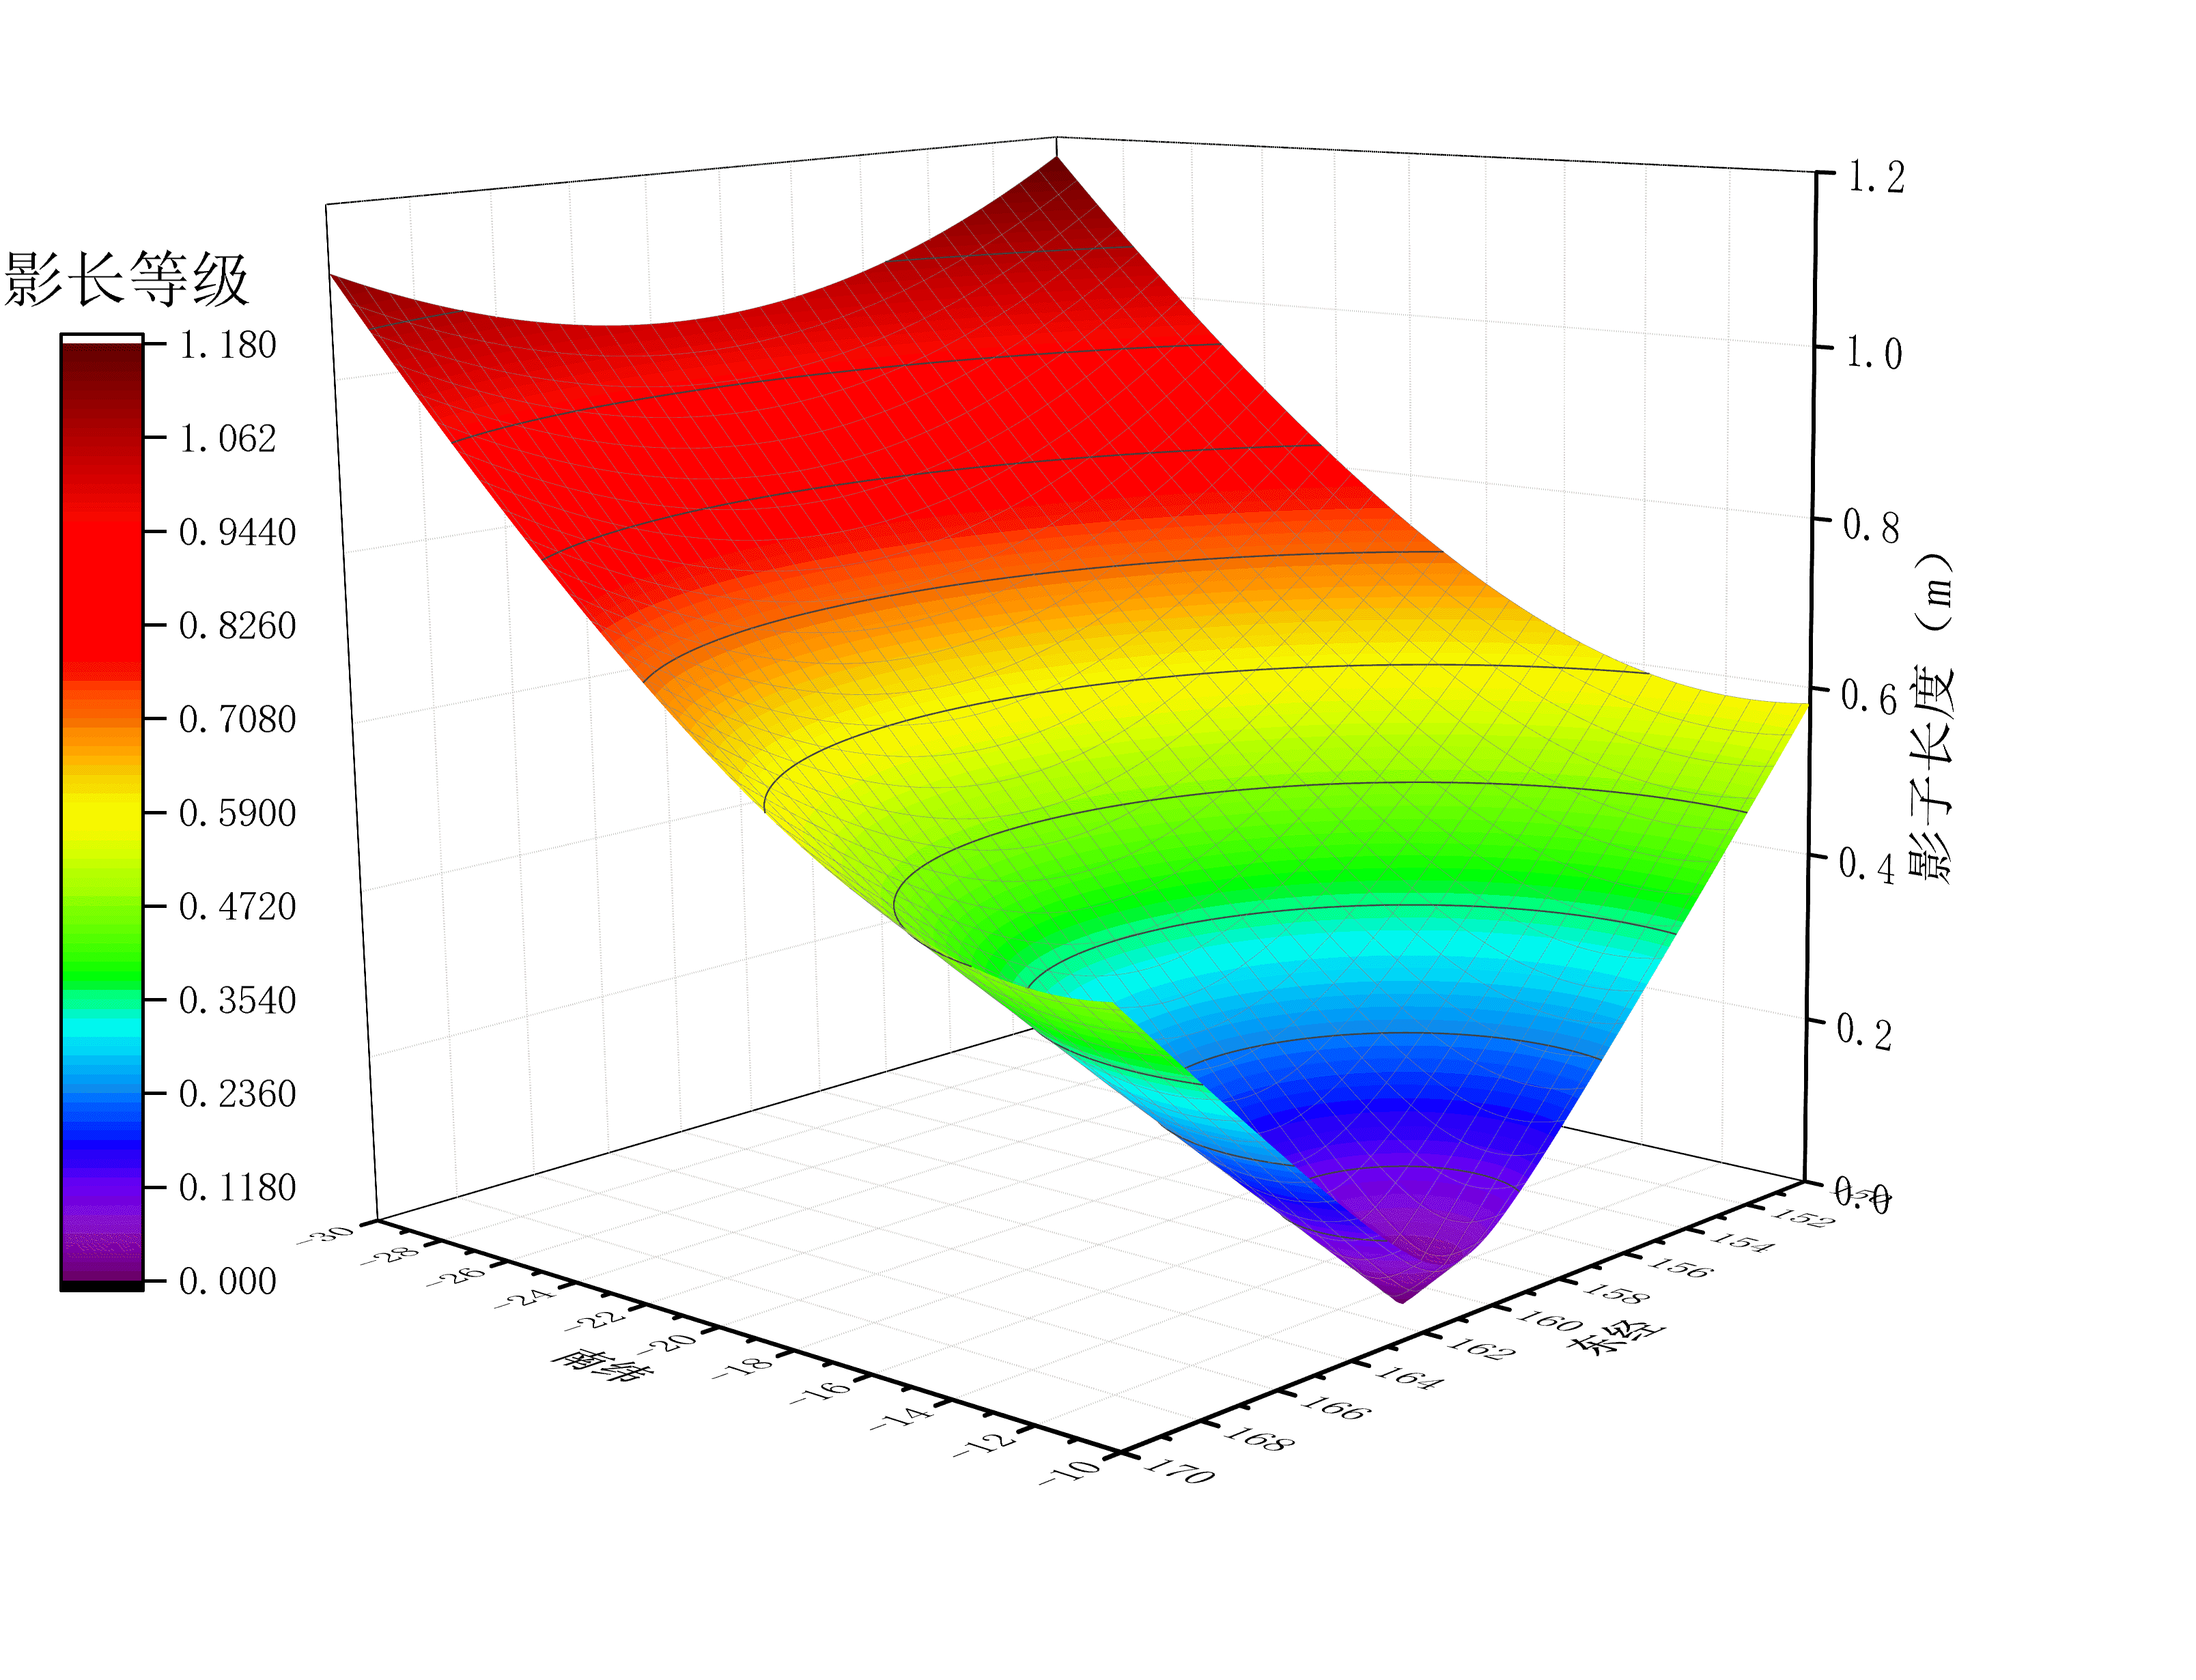
\includegraphics[scale=0.4]{images/jingwei.png}
  	     	\caption{经纬度对太阳影子长度的影响}
  	     	\label{jingwei}
  	     \end{figure}   	       
\end{enumerate}




\subsubsection{影子长度变化模型的求解与分析}
将问题一中具体参数:$year=2015$,$N=295$天(10月22日),$t\in[9,15]$(小时),以及\[L=3,\psi=\frac{39.9072222\pi}{180},\phi=\frac{116.391389\pi}{180}\]代入上述影子长度变化模型可得太阳影子长度随当地北京时间$t$的变化曲线如图~\ref{yingchang}~所示。从图中可以看出影长变化的趋势为先减后增,在北京时间12.2时达到正中午,影长最短。为了看出一整天中影子变化规律,我们将横坐标范围加大,绘制出图~\ref{yingchangtian}~。图中两个峰值分别对应着日出和日落时影长会发生突变的现象,而峰值的不同说明早上和下午是有区别的,图~\ref{yingchang}~中影长关于极小值点所在纵轴并不对称(说明函数不是二次函数)亦说明了这一点。我们默认太阳高度角$\alpha$是大于0的,对于图~\ref{yingchangtian}~中位于0以下的曲线部分实际上并无意义。

\begin{figure}[h]
	\centering
	\begin{minipage}{.45\textwidth}
		\centering
		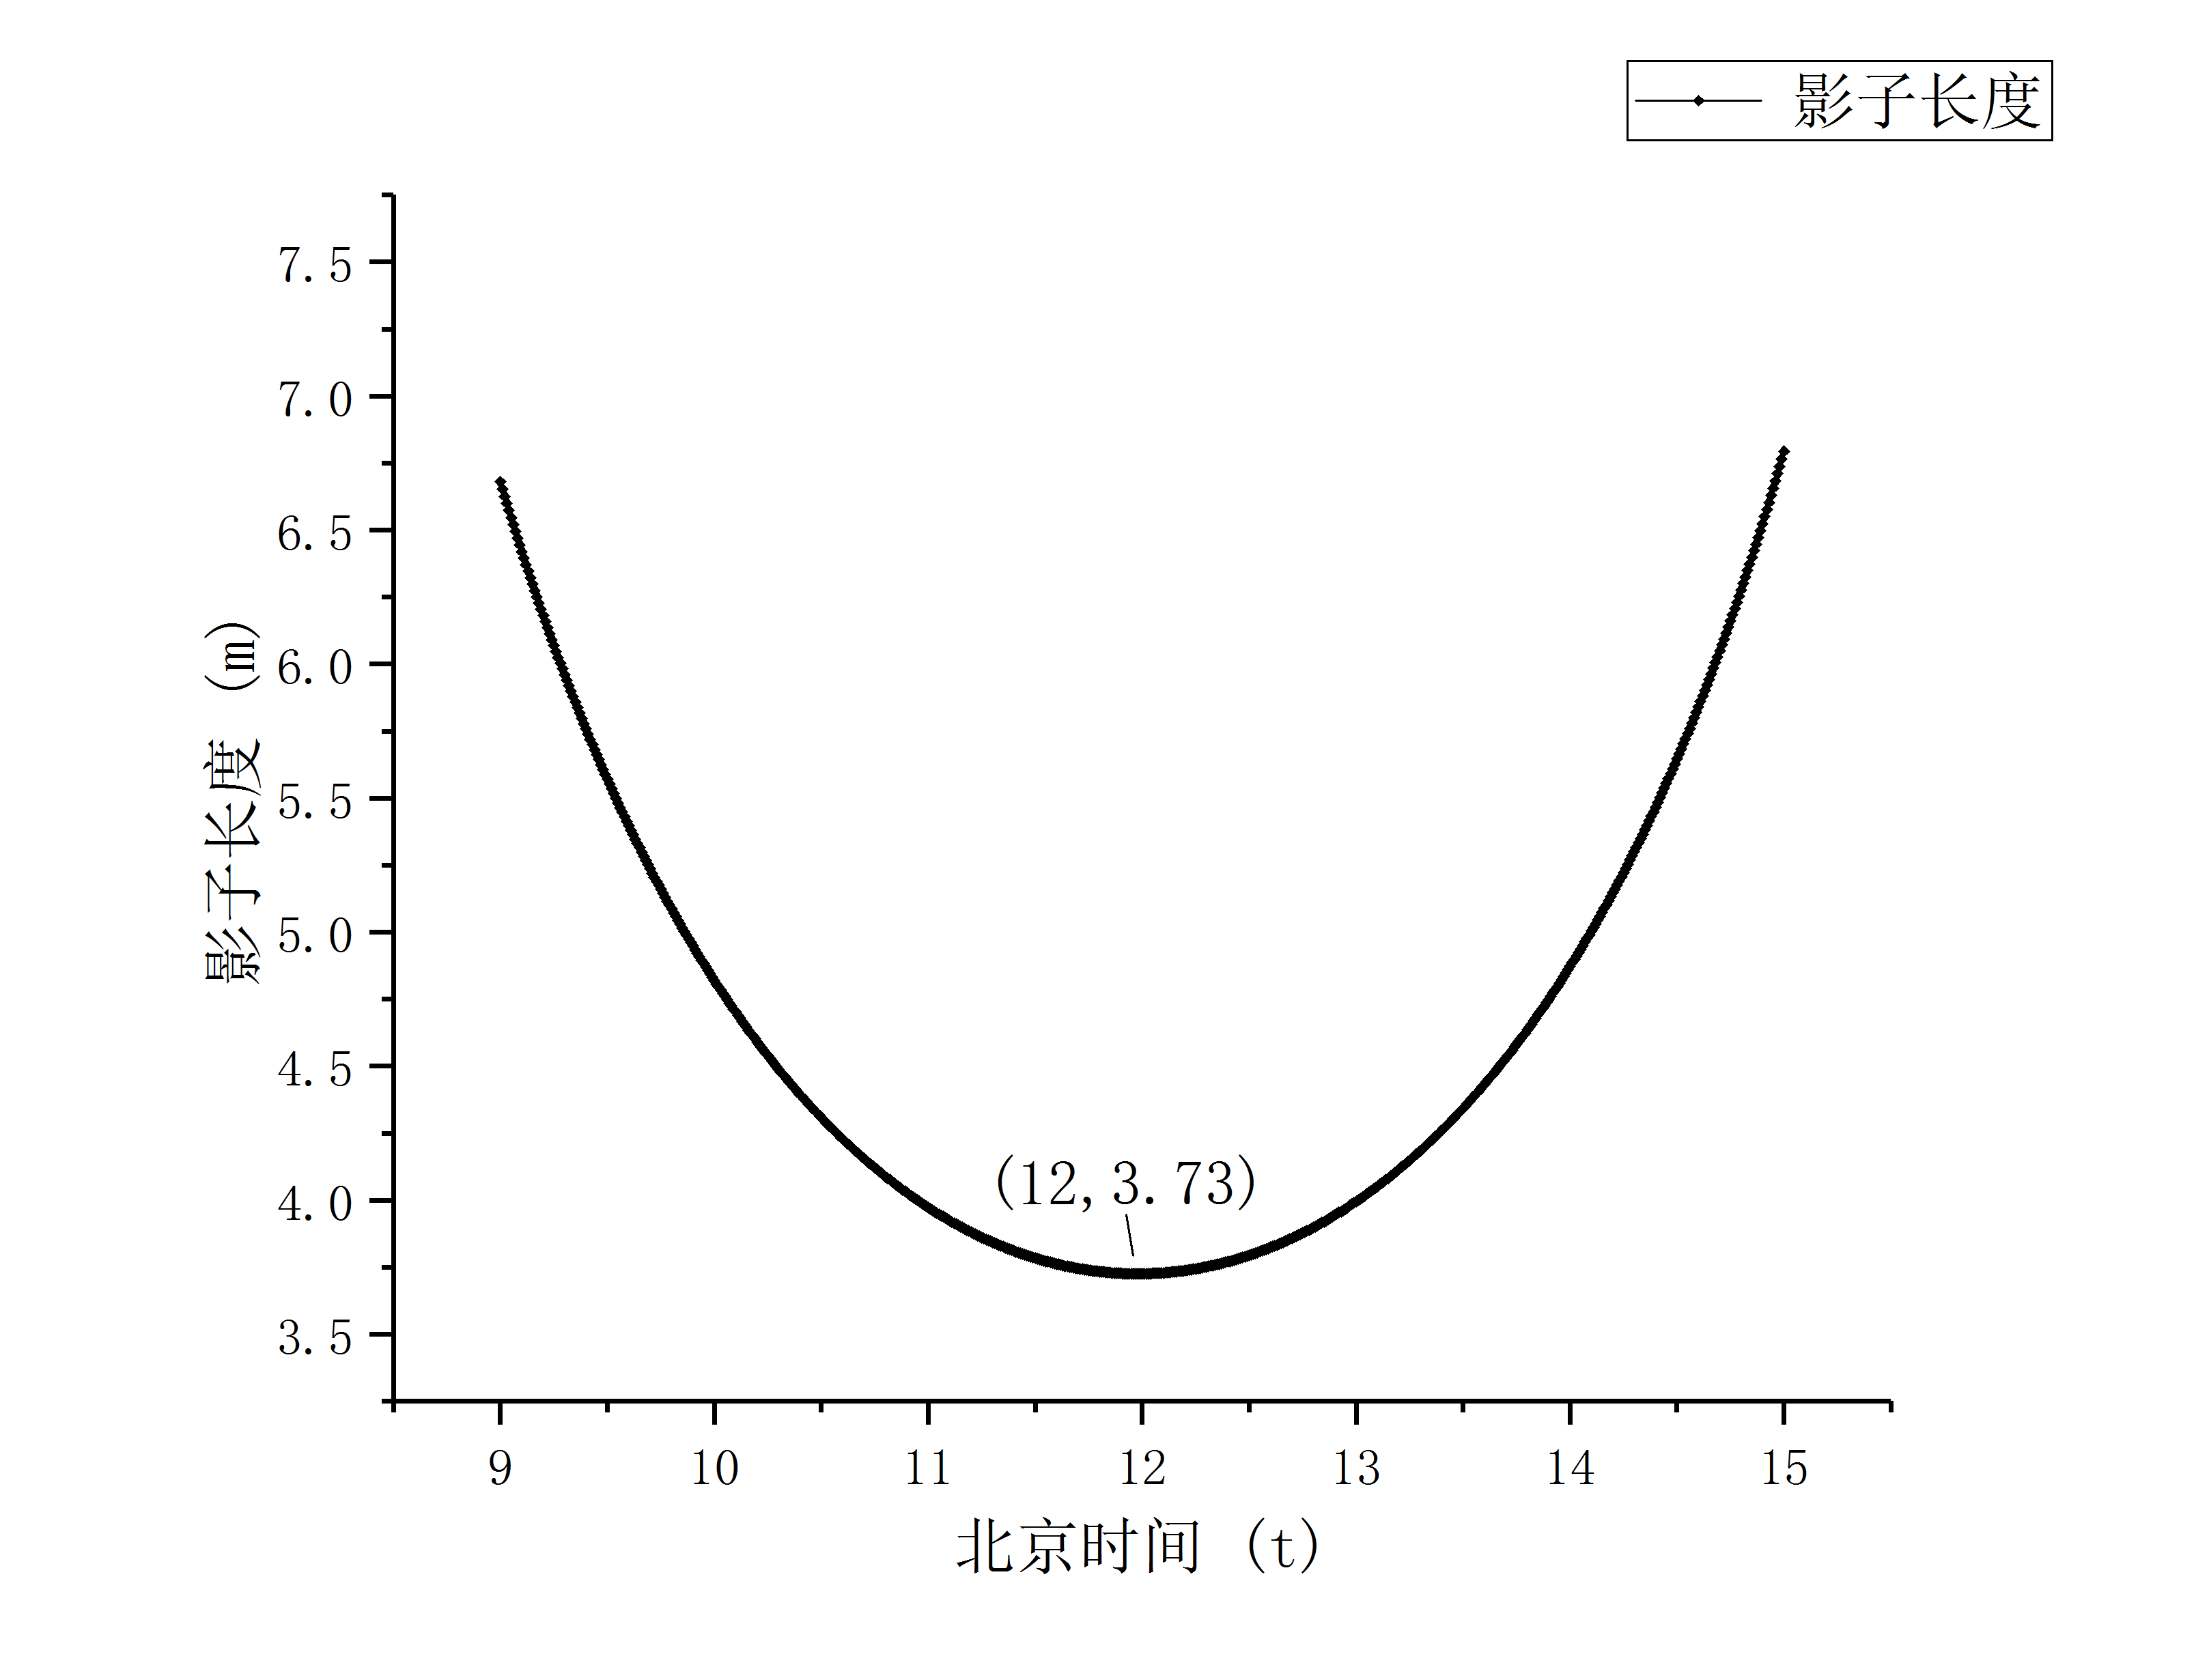
\includegraphics[width=.95\textwidth]{images/yingchang.png}
		\caption{太阳影子长度变化曲线}
		\label{yingchang}
	\end{minipage}\hfill
	\begin{minipage}{.45\textwidth}
		\centering
		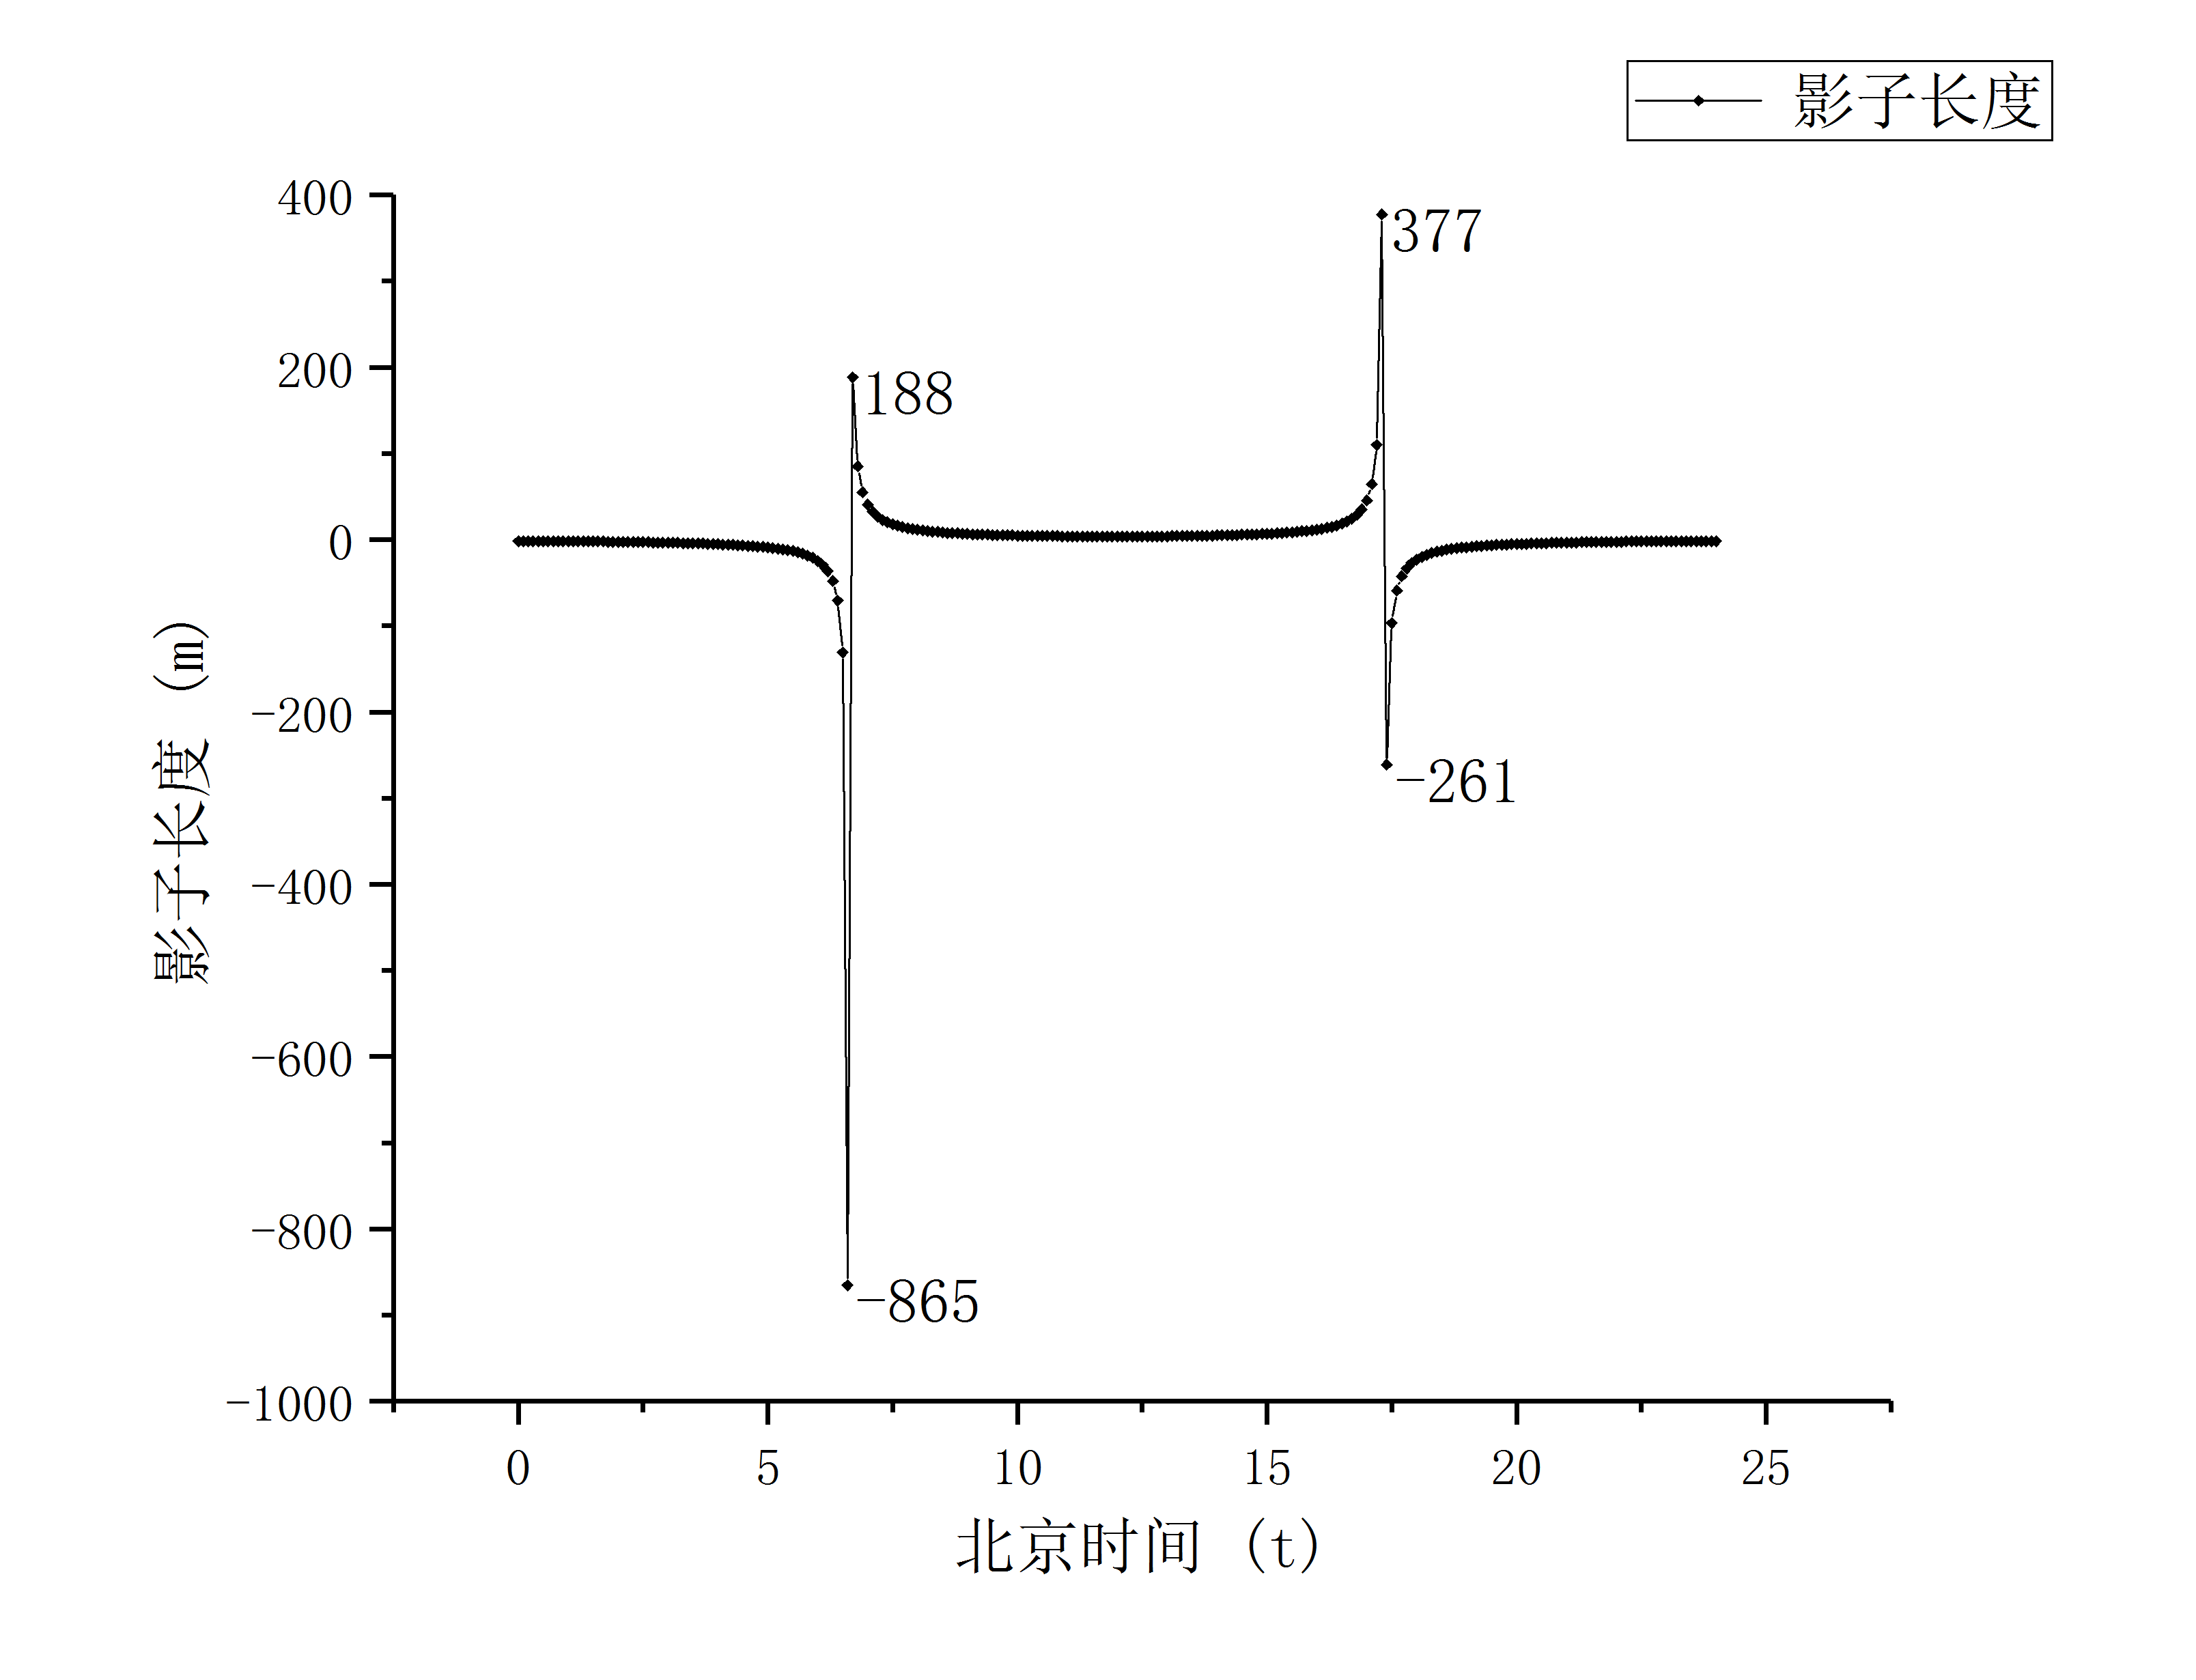
\includegraphics[width=.95\textwidth]{images/yingchangtian.png}
		\caption{全天影子长度变化曲线}
		\label{yingchangtian}
	\end{minipage}	
\end{figure}



\subsection{问题二直杆地点反演模型的建立与求解}
\subsubsection{直杆地点反演模型的建立}
分析问题二可知,此处的未知量有经度$\phi$、纬度$\psi$、杆长$L$、北京时间$t$、影子长度$l$。而拍摄地的地理位置由经纬度确定,由问题一中模型经纬度可以表示为:
\begin{equation}
(\phi,\psi)=f(L,t,l)  
\end{equation}
由地理知识易知当某地的真太阳时等于12时,影子长度达到最小。经度$\phi_0=120^\circ$的地方在北京时间$t_0=12$点时影子长度最小。从而,如若知道某地白天影子最短时的北京时间$t^{'}$,便可以通过下式求出当地经度。
\begin{equation}
\frac{\phi-\phi_0}{15^\circ}=t^{'}-t_0   \label{suanjingdu}
\end{equation}
为确定当地白天的影子长度变化关系,利用附件一中的数据可以得到不同时刻的21个影长($l_i,i=1,2,\cdots,21$),在此基础上,结合问题一中的函数关系并利用三角函数拟合(见 $5.2.2$)可得影长与北京时间的变化关系$l(t)$。利用MATLAB可求得$l(t)$的极小值与极值点(白天内只有一个极值),从而求得经度$\phi$。此时,只需要确定纬度即可,纬度的函数为:
\begin{equation}
\psi=f(L,t,l)
\label{llt}
\end{equation}

为求得最可能的地点,亦即找出影子长度与附件一中21组数据最为接近的地方。为此,基于最小二乘法的思想建立目标函数:
\begin{equation}
\min \quad \Delta L = \sum\limits_{i = 1}^{21} ({l_i}-l_{t_i})^2
\end{equation}
其中,$l_{t_i}$表示在任意给定一组$(\psi,L)$情况下,当地北京时间为$t_i$时的的影长计算值。计算式为$l_{t_i}=g(\psi,L,t_i)$,函数$g$的表达式由公式\ref{llt}确定。

\subsubsection{拟合三角函数的确定}  
由问题一中可知影子长度$l$与北京时间$t$的关系满足:
\begin{align}
l(t)=&\frac{L\sqrt{1-(sin\alpha)^2}}{sin\alpha}  \notag \label{lalpha} \\
sin \alpha=&sin \psi sin\delta +cos \omega cos \psi cos \delta \notag
\end{align}
本问中拍摄日期(4月18日)已经给定,亦即积日$N=108$天已经给定,由公式\ref{deta}可知太阳赤纬角$\delta$是定值。而对于给定的某地、给定的直杆,纬度$\psi$、杆长$L$亦应该为一定值。从而决定$l$的只有$\omega$,而
\[\omega=\pi (\frac{T_c}{12}-1),T_c=t+\Delta t\]
可知$\omega$与北京时间$t$为一次函数关系。从而不难待定
\[sin \alpha =A_2cos(\pi(\frac{t}{12}-b_2))+b_1\]
其中,$A_2 \in [-1,1],b_1 \in [-1,1]$。基于以上分析,利用待定系数法可以给定拟合函数
\begin{equation}
l_1=\frac{A_1\sqrt{1-(A_2cos(\pi(\frac{t}{12}-b_2))+b_1)^2}}{A_2cos(\pi(\frac{t}{12}-b_2))+b_1}
\end{equation}
其中,$A_1,A_2,b_1,b_2$为需要拟合的参数。并且它们满足以下几式:
\begin{align}
|A_1|=&L  \\ \label{niding1}
|b_1|=&|sin\psi sin\delta |  
\end{align}

可通过Origin 自定义拟合函数拟合非线性曲线求解。

\subsubsection{直杆地点反演模型的求解}  
\subsubsubsection{拟合函数的求解}
$\qquad$在Origin中自定义好拟合函数后对附件一中的影长进行拟合,参数设置如表~\ref{canshu1}~。
\begin{table}[!htbp]
	\centering
	\caption{Origin 非线性拟合参数设置}\label{canshu1}
	\begin{tabular}{ccc}
		\toprule[1.5pt]
		迭代算法& 容差 &加权方式\\
		\midrule[1pt]
        正交距离回归&$1 \times 10^{-14}$ &不加权\\
		\bottomrule[1.5pt]
	\end{tabular}
\end{table}
利用Origin的迭代算法拟合时发现正交距离回归效果较好,文献中给出了其与最小二乘法的误差对比,正交回归更具优势。容差是给定数据和当前拟合函数之间加权距离相对变化的最小约束。如果拟合过程中的相对变化低于预先设置的容差,拟合过程将停止。加权方式是指对所给数据中各个数据的偏重程度,不加权相当于认为附件一所给21组数据地位平等。

经迭代收敛后得到报告如图~\ref{nihe1}~、表\ref{baogao1}所示。

 \begin{figure}[h]
	\centering
	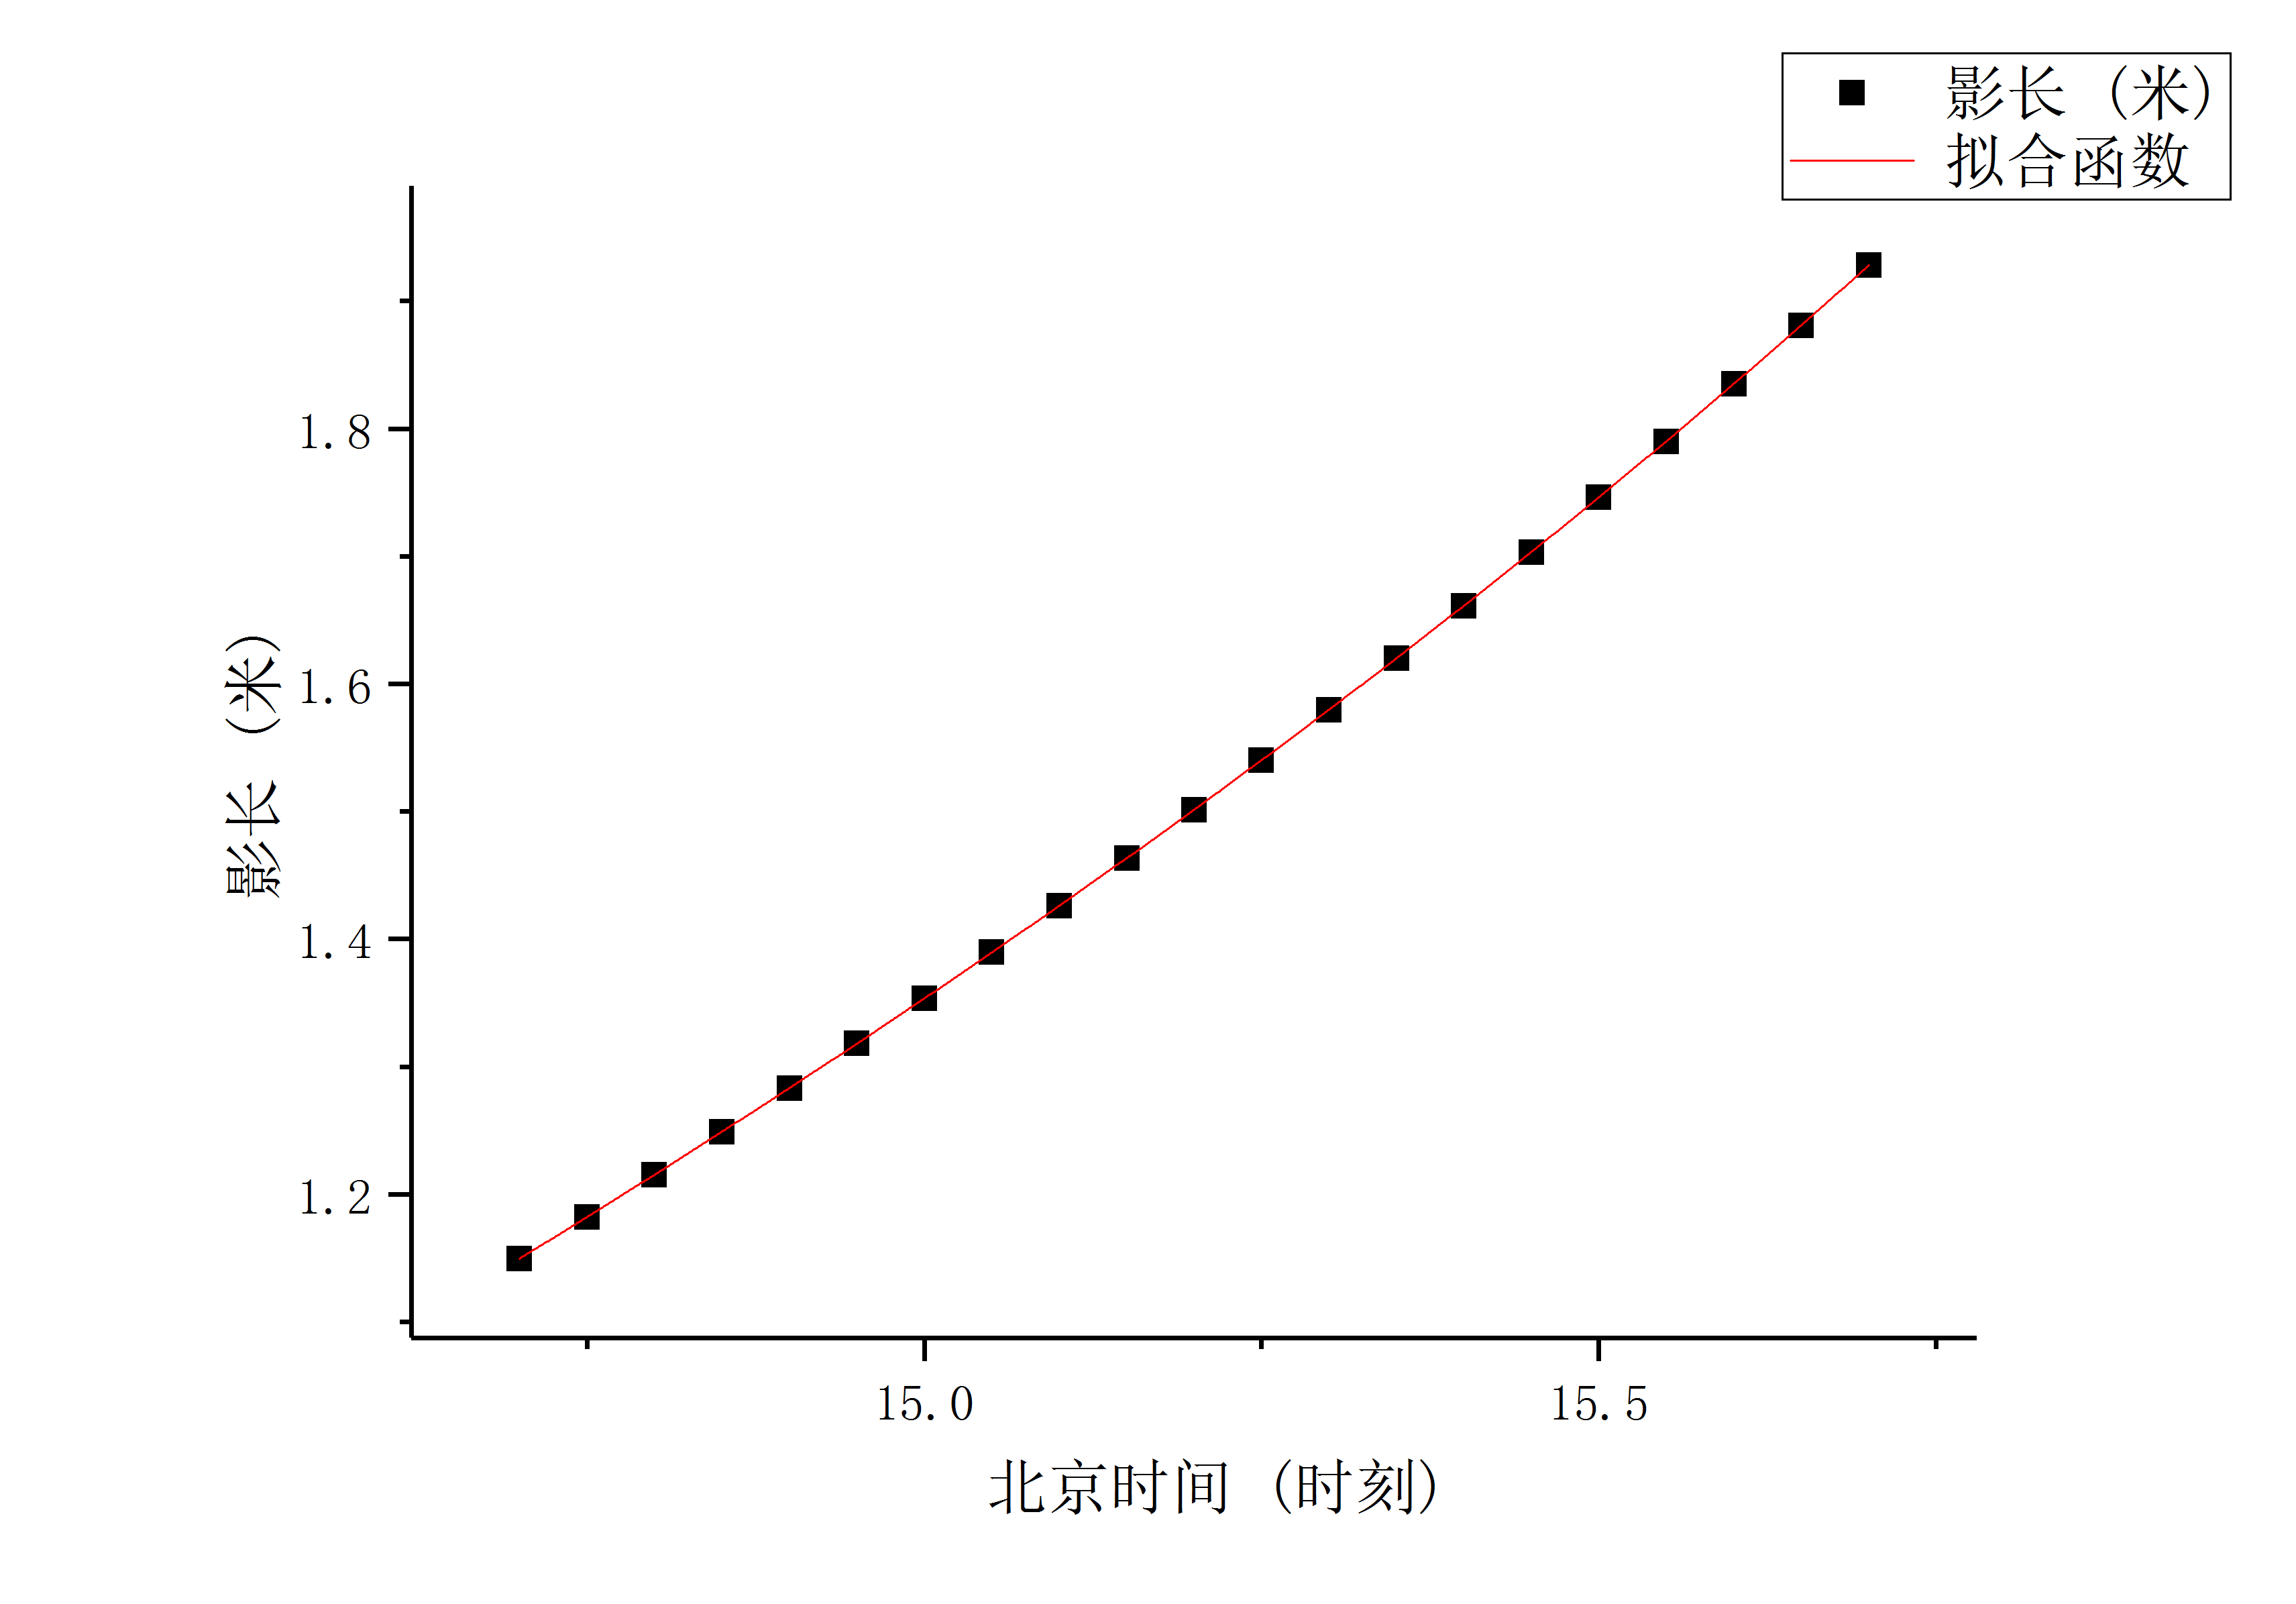
\includegraphics[scale=0.4]{images/niheyi.png}
	\caption{拟合结果报告}
	\label{nihe1}
\end{figure}  
\begin{table}[!htbp]
	\centering
	\caption{函数拟合参数报告}\label{baogao1}
	\begin{tabular}{cc}
		\toprule[1.5pt]
		参数& 值 \\
		\midrule[1pt]
	A1	&$-2\pm  0.01123$\\
	A2	&$-0.92184 \pm  0.00204$\\
	b1	&$-0.06992 \pm 0.00315$\\
	b2  &$	1.05746\pm  0.00178$\\
	Reduced Chi-Sqr &$	1.11508\times 10^{-9}$\\
	R平方(COD)&	1\\
		\bottomrule[1.5pt]
	\end{tabular}
\end{table}
从表\ref{baogao1}中可以看出看出拟合效果非常好。四个参数的误差范围均十分小,最大的波动仅达0.011;Reduced Chi-Sqr 指加权卡方检验系数,表示数据点和拟合函数相应点差的平方和,这个值越接近于零越好;$R^2$表示决定系数,在$[0,1]$之间变化,越接近于1越好。


我们知道,一般的函数拟合(通常不知道原函数的结构)仅在给定数据区间具有较好的近似效果。但是本文的拟合函数是根据影子长度的具体函数结构构造而来,可以比较好的近似整个区间上函数值。为此,我们画出由上述参数确定的拟合函数$l_1$在中午区间与一整天24小时区间的函数图像如图~\ref{yanzheng2}~、~\ref{yanzheng1}~所示
\begin{figure}[h]
	\centering
	\begin{minipage}{.45\textwidth}
		\centering
		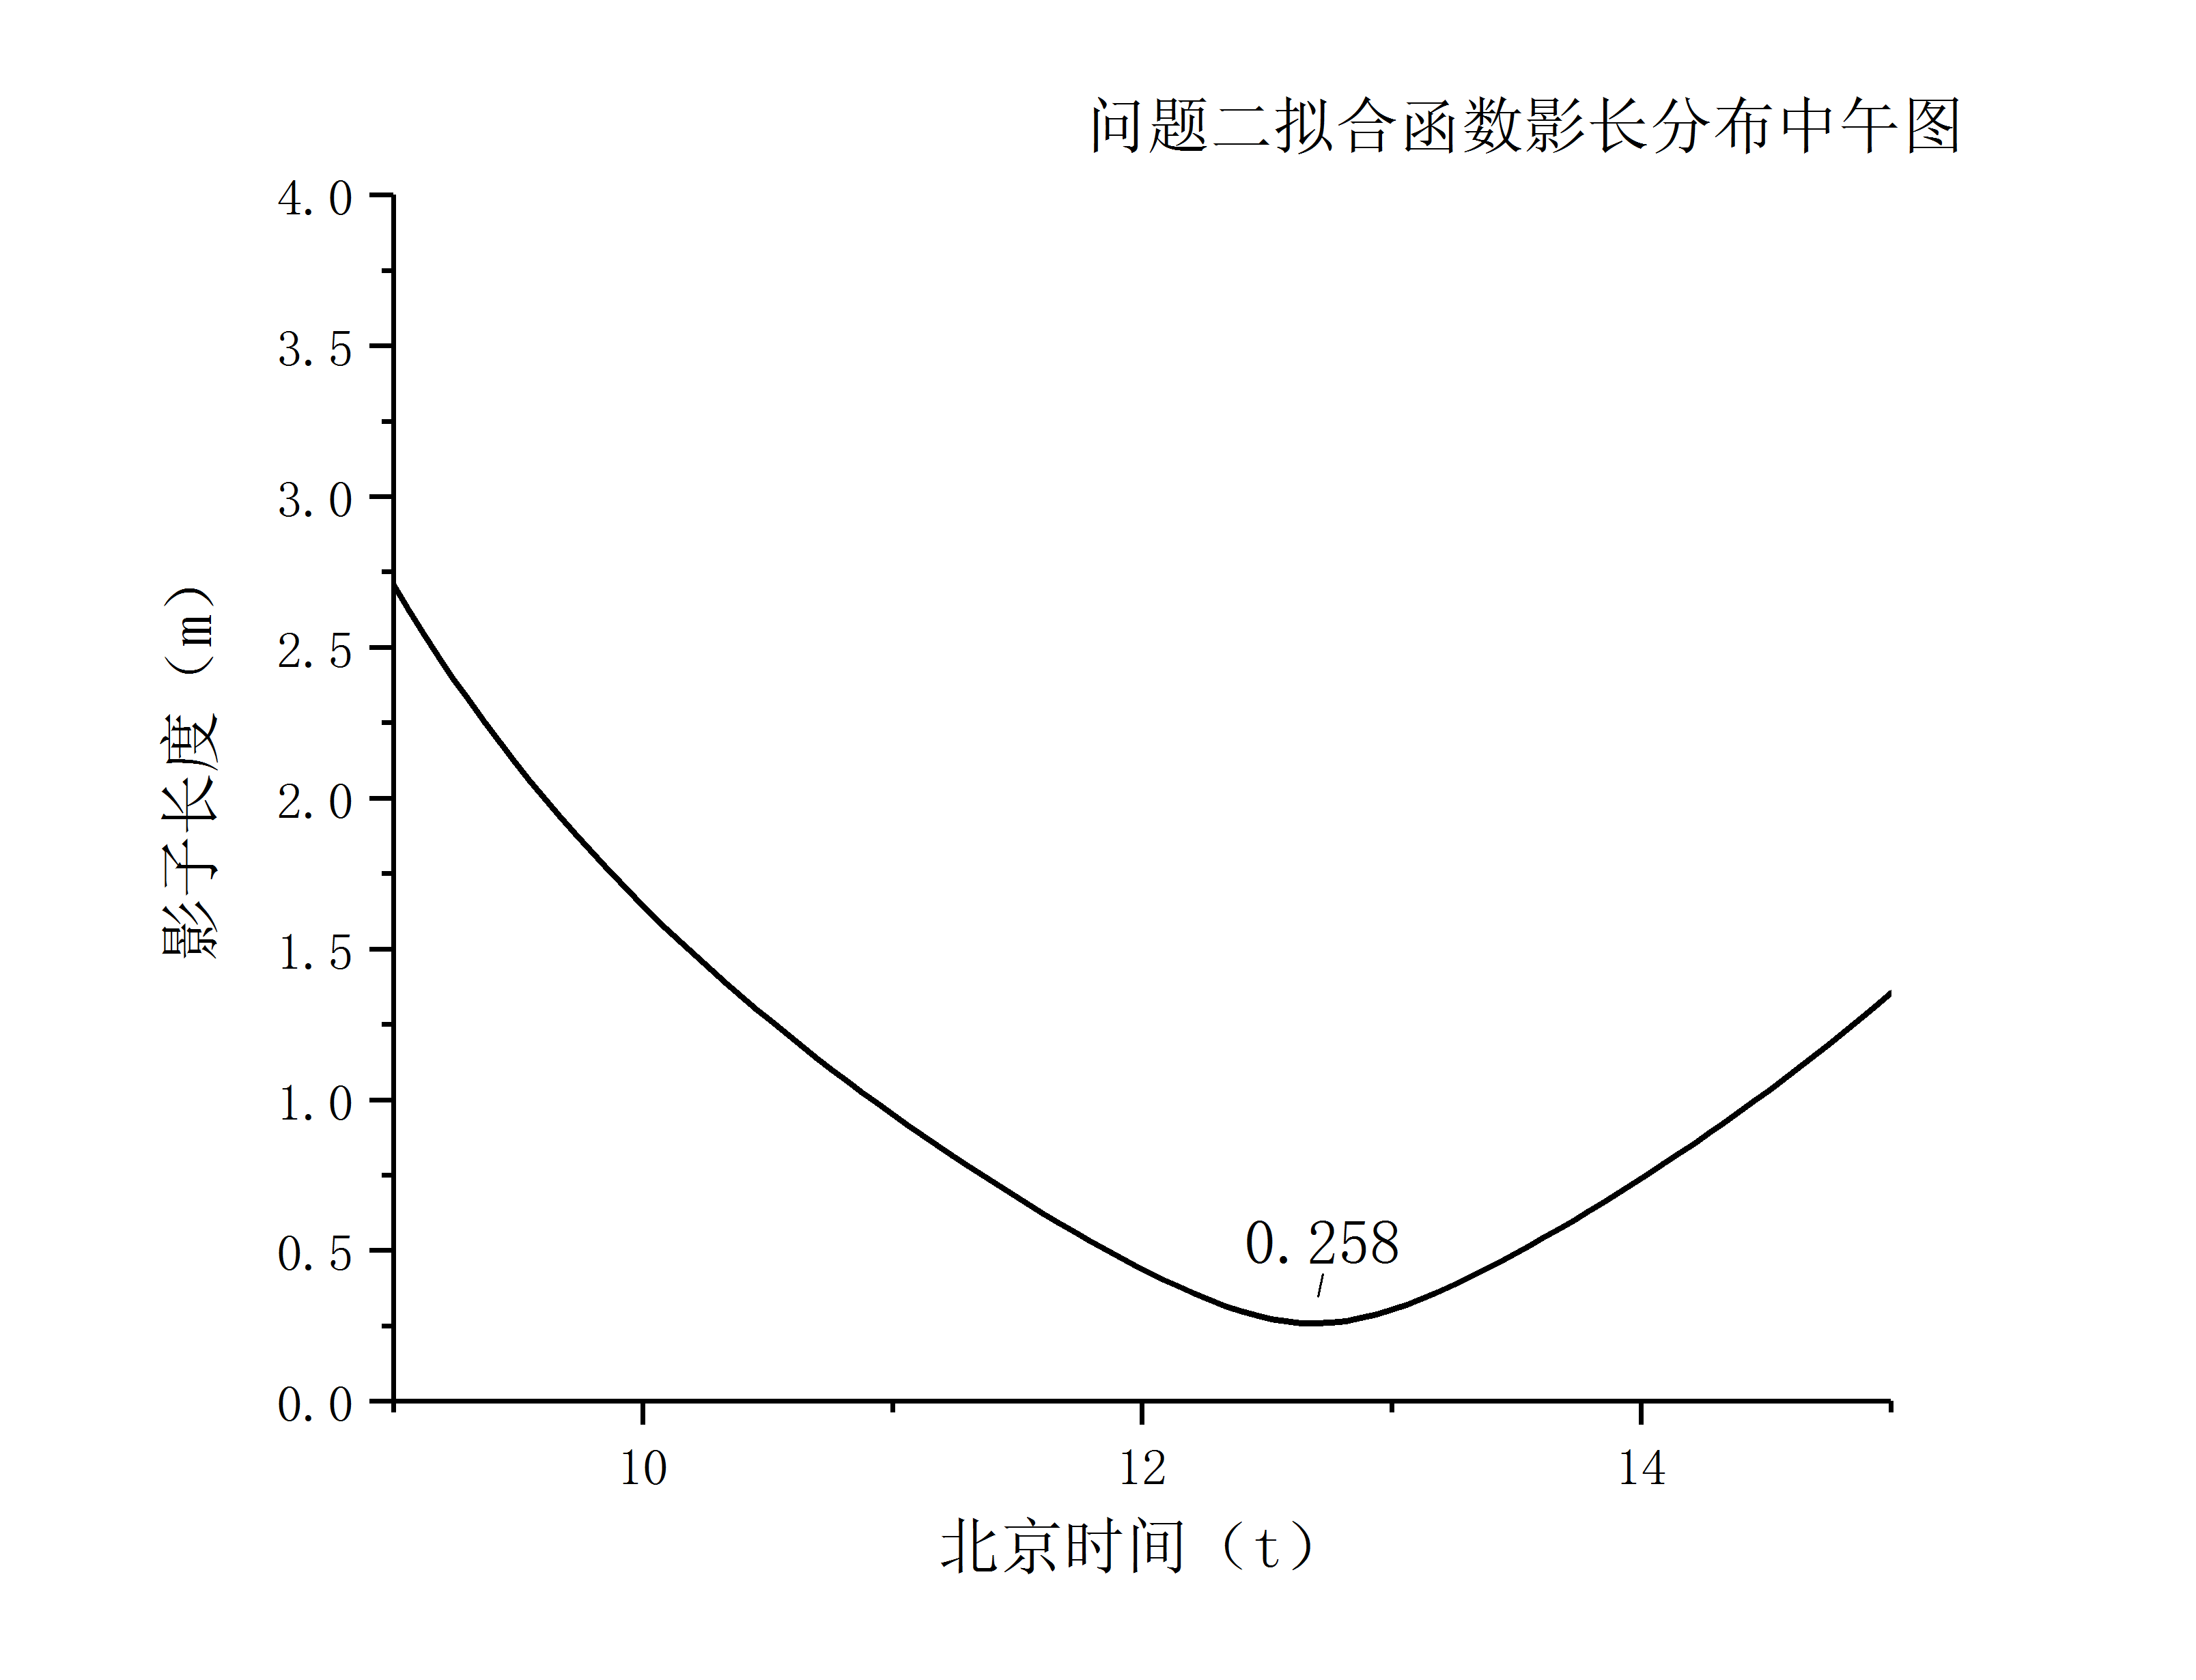
\includegraphics[width=.95\textwidth]{images/yanzheng2.png}
		\caption{拟合函数中午影长曲线图}
		\label{yanzheng2}
	\end{minipage}\hfill
	\begin{minipage}{.45\textwidth}
		\centering
		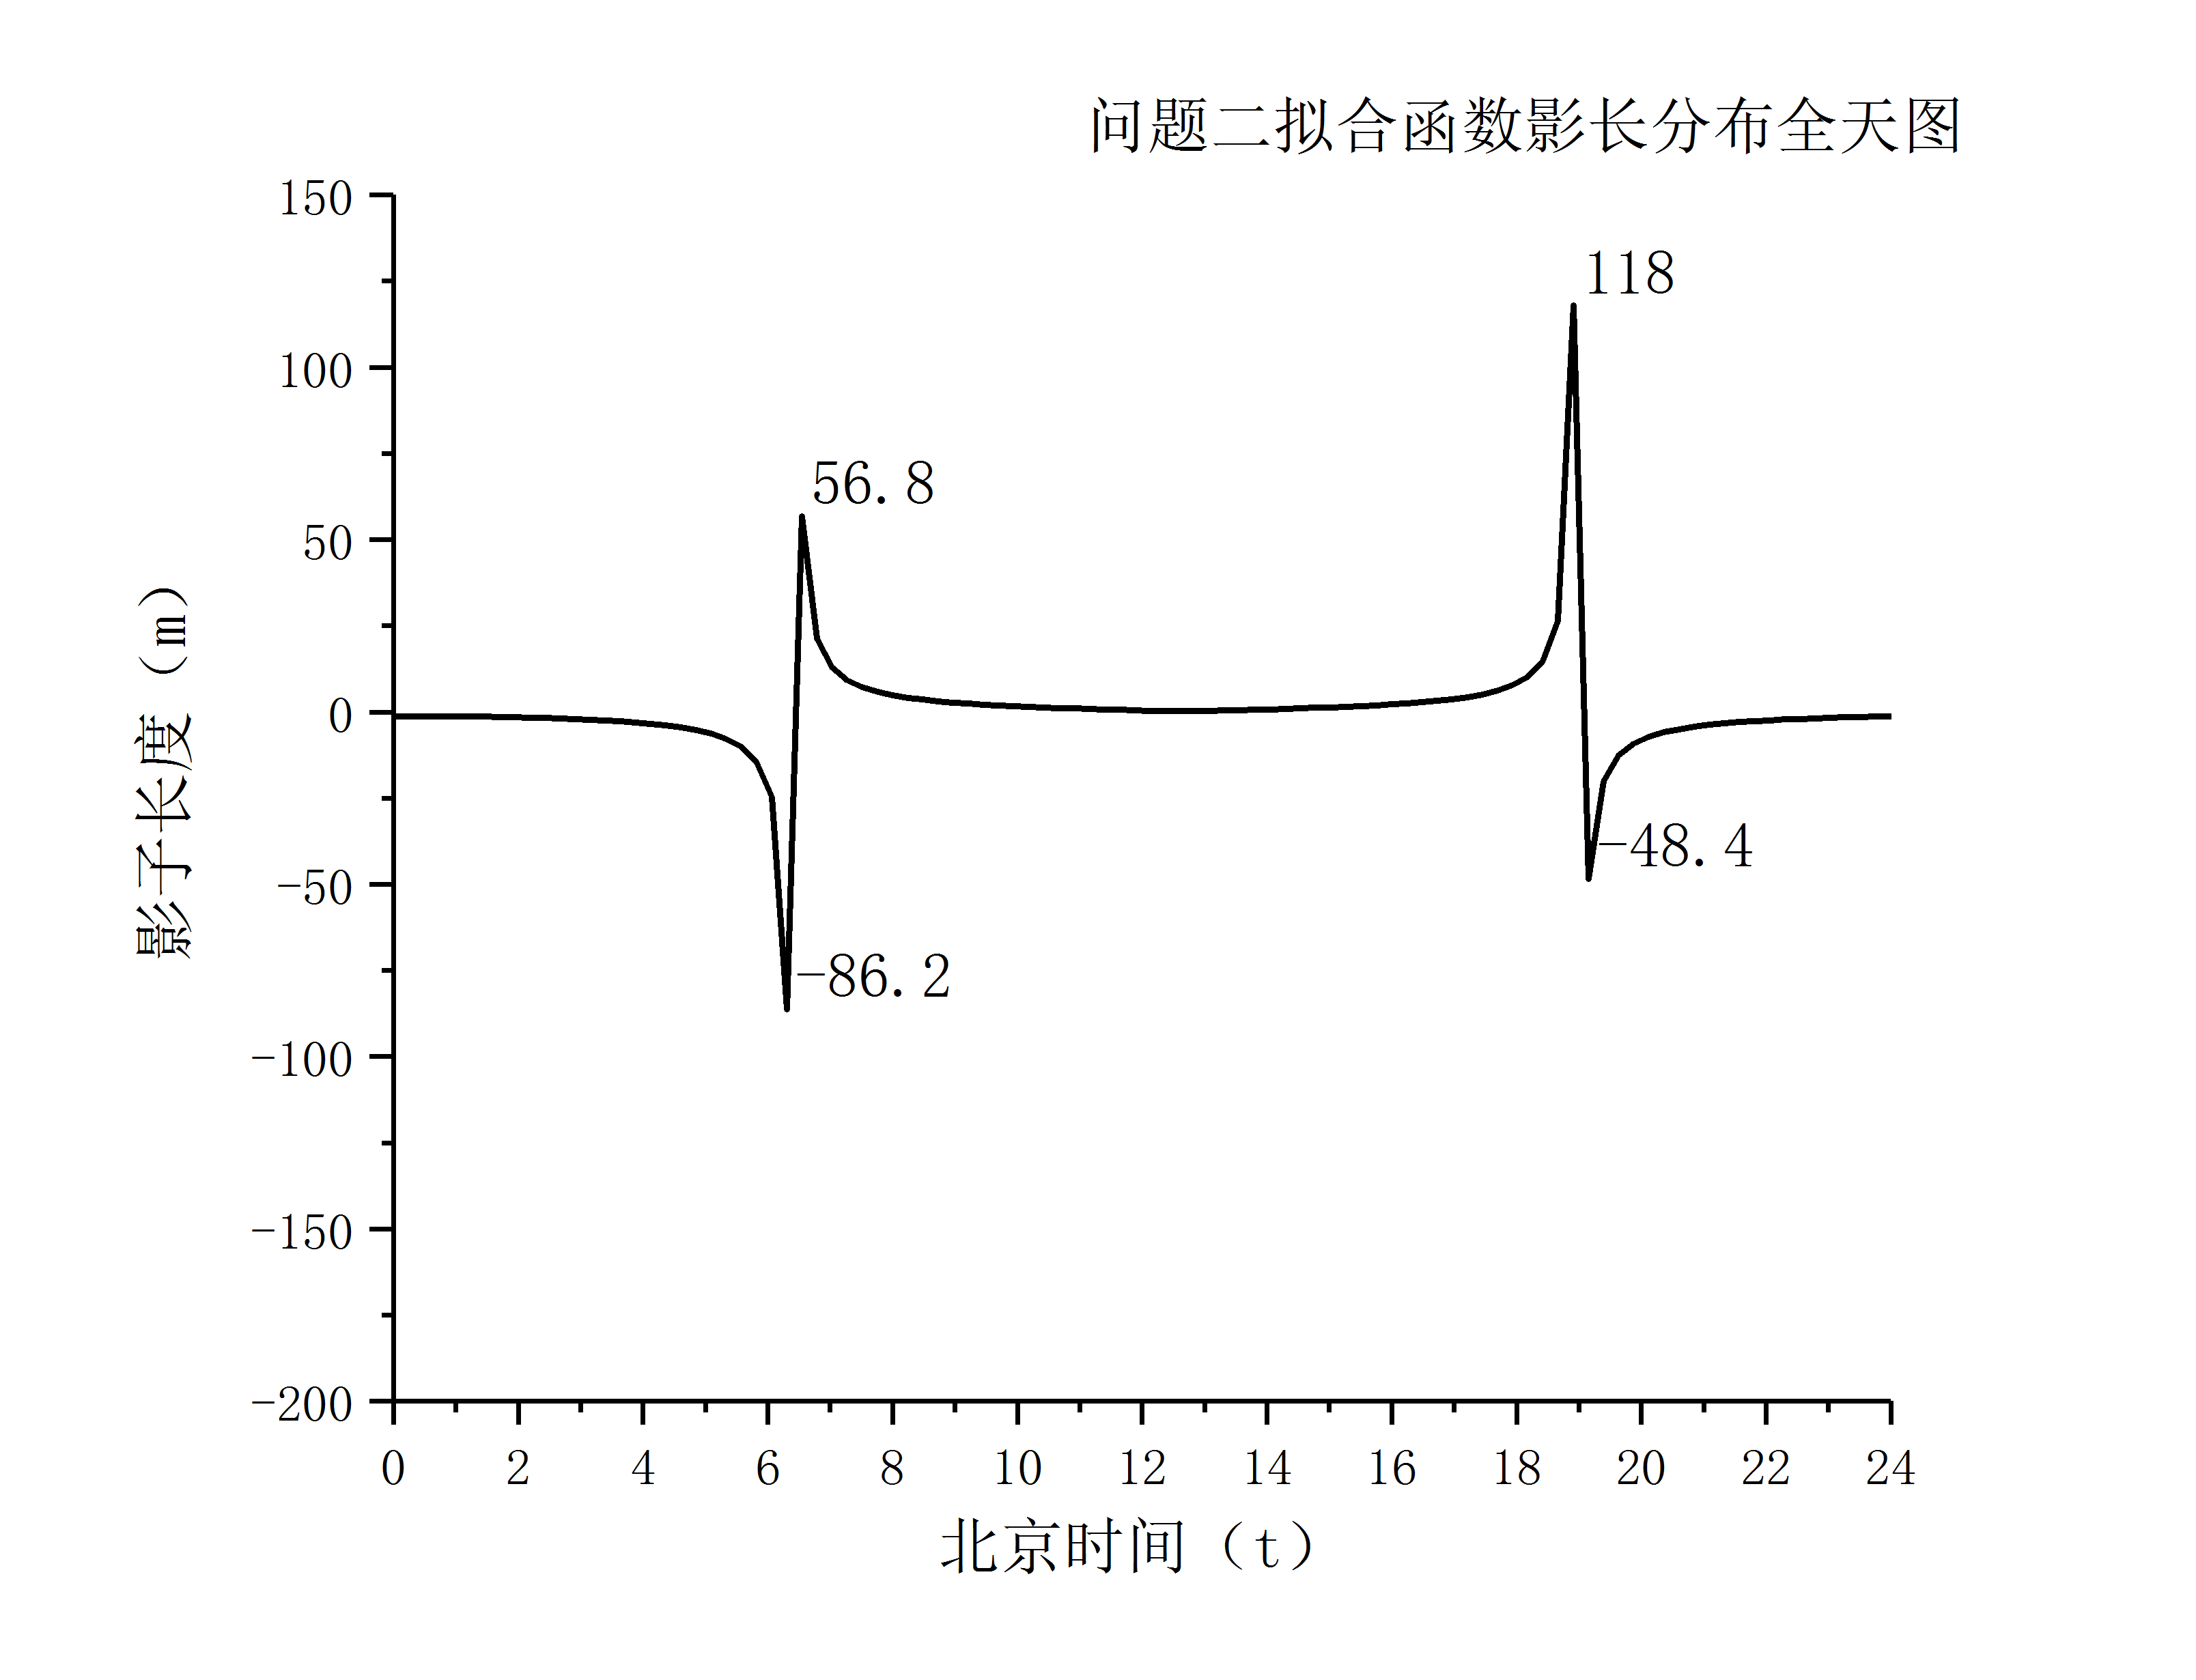
\includegraphics[width=.95\textwidth]{images/yanzheng1.png}
		\caption{拟合函数全天影长曲线图}
		\label{yanzheng1}
	\end{minipage}	
\end{figure}
对比图~\ref{yingchang}~~、\ref{yingchangtian}~发现,此拟合函数$l_1$与问题一求解出的函数趋势、形状几乎一模一样,唯一不同点仅在于拟合的函数在日出、日落的峰值大小不一样。

基于此拟合函数的高度近似,我们完全可以不仅仅局限于用它来求解经度。容易计算$sin \delta=0.1824$,而$b_1=-0.06992$。由拟合函数的系数满足的公式\ref{niding1}可得 $\psi=22.5382^\circ$且$L=2$。故而可以推测这两个值应该是下文的一个理想解。亦即下文求出来的部分杆长解应该在2米左右,部分纬度解应该在$22.5382^\circ$左右。

\subsubsubsection{直杆地点反演模型的求解与分析}
由上述拟合方法已经确定了拟合函数$l(t)$。利用MATLAB可以求得白天中影子最短的北京时间为 12.6895,最短影长为$0.2583$米。将最短时间代入公式\ref{suanjingdu},可得$\phi=109.6575^\circ$。从而我们的目标变成了以下的一个两个自变量的单目标优化问题:
\begin{align}
\min \quad \Delta L = &\sum\limits_{i = 1}^{21} ({l_i}-l_{t_i})^2 \notag\\ 
l_{t_i}=&g(\psi,L,t_i),i=1,2,\cdots,21 \notag\\
L \in& (0, + \infty )\notag \\
\psi  \in& ( - \frac{\pi }{2},\frac{\pi }{2})  \notag
\end{align}
本文采用遗传算法求解,经尝试后调节好参数。程序单独运行30次为一组,一共运行十组,结果如表~\ref{answer1}~所示。

\begin{table}[!htbp]
	\centering
	\caption{遗传算法所得结果}\label{answer1}
	\begin{tabular}{ccc}
		\toprule[1.5pt]
		纬度& 杆长&适应度函数量级 \\
		\midrule[1pt]
	18.4120 &   1.9671 &   -6\\
	18.4144 &   1.9671  &  -6\\
	-0.1331  &  1.8479   & -6\\
	-0.1299  &  1.8480  &   -6\\
	-0.1313&    1.8479  &   -6\\
	18.4137  &  1.9671   &  -6\\
	-0.1302  &  1.8480  &   -6\\
	18.4150 &   1.9671   &  -6\\
	18.4148  &  1.9671   &  -6\\
	-0.1319  &  1.8479   &  -6\\
		\bottomrule[1.5pt]
	\end{tabular}
\end{table}

从表中可以看出基本只有两个较优纬度:$18.41^\circ$和$-0.13^\circ$。并且杆长与预测值2米十分接近,而纬度$18.41^\circ$与$22.5382^\circ$亦相差不大。预测的如此准确归根结底是因为附件一所提供的数据十分可靠,使得根据问题一中函数结构拟合的函数极高的还原了原来函数的特质。附件一所提供数据为4月18日,太阳直射北半球,遗传算法求出的两个较优纬度基本关于直射纬度对称。故而可以推测最可能的地点为:海南岛三亚和西加里曼丹。


\subsection{问题三直杆地点反演模型的建立与求解}
\subsubsection{直杆地点反演模型的建立}
分析问题三可知,此问关键在于在第二问的基础上增加了积日$N$这一个未知量。由上述公式可知与$N$有关的公式有\[\delta=\frac{469\pi sin(\frac{2\pi(N+284)}{365})}{3600}  \]
即积日变化会引起太阳赤纬角$\delta$的变化。因此,为了保证拟合的高度近似,需要对问题二中的拟合函数进行改进。

当引入一个新的变量$N$后,问题二中的纬度函数$l_{t_i}$的函数变为:
\begin{equation}
l_{t_i}=\varphi(\psi,L,t_i,N)
\end{equation}
基于问题二中同样的思想,在求得经度$\phi$的前提下。我们建立目标函数:
\[\min \quad \Delta L = \sum\limits_{i = 1}^{21} ({l_i}-l_{t_i})^2\]
其中,$l_{t_i}$表示在任意一组($\psi,L,N$)情况下当地北京时间为$t_i$时的影长计算值。
\subsubsection{拟合三角函数的改进}
显然对拟合函数的改进关键在于公式\[sin \alpha=sin \psi sin\delta +cos \omega cos \psi cos \delta \]
的待定。在充分考虑上式中的变量以及公式\ref{deta}可以给出如下待定:
\begin{equation}
sin\alpha=A_2cos(k_1sin(b_3))cos(k_2 t-b_1)+b_2sin(k_2sin(b_3))
\end{equation}
从而最终确定的拟合函数为
\begin{equation}
l_1=\frac{A_1\sqrt{1-(A_2cos(k_1sin(b_3))cos(k_2 t-b_1)+b_2sin(k_2sin(b_3)))^2}}{A_2cos(k_1sin(b_3))cos(k_2 t-b_1)+b_2sin(k_2sin(b_3))}
\end{equation}
上式中,$A_1,A_2,b_1,b_2,b_3$为需要拟合的参数,$k_1=0.4093,k_2=0.2618$。同问题二,这些参数满足以下几式:
\begin{align}
|A_1|=&L  \\
|A_2|=&|cos\psi|  \\
b_3=&\frac{2\pi (N+284)}{365}\pm 2k\pi  ,k \in Z
\end{align}
并且$b_2\in[-1,1],A_2 \in [-1,1]$。此拟合不仅可以求出经度$\phi$,由此3式还可以分别给出杆长、纬度、积日的预测值。

\subsubsection{直杆地点反演模型的求解与分析}
\subsubsubsection{附件二数据对应模型的求解与分析}
$\qquad$Origin拟合报告如表~\ref{baogao2}~。可见拟合效果仍旧非常好,最高参数误差仅达4.7且$R^2=1$。在MATLAB中求出此函数在北京时间 14.6876时达影长最小值 0.6934米。从而计算得到经度$\phi=79.6857^\circ$。
\begin{table}[!htbp]
	\centering
	\caption{附件二函数拟合报告}\label{baogao2}
	\begin{tabular}{cc}
		\toprule[1.5pt]
		参数& 值 \\
		\midrule[1pt]
		A1	&$-1.99099 \pm 0.01463$\\
		A2	&$	0.7678 \pm 0.27691$\\
		b1	&$0.70362\pm 0.00157$\\
		b2  &$-1 \pm2.72981$\\
     	b3  &$1.04044 \pm 4.74445$\\
		Reduced Chi-Sqr &$9.24525\times10^{-10}$\\
		R平方(COD)&	1\\
		\bottomrule[1.5pt]
	\end{tabular}
\end{table}
为了确保在此拟合下是否仍能准确预测杆长、纬度、甚至积日,我们画出拟合出的函数影子长度变化曲线如图\ref{yanzheng3}、\ref{yanzheng4}与问题一中的图\ref{yanzheng2}、\ref{yanzheng1}进行对比。

\begin{figure}[h]
	\centering
	\begin{minipage}{.45\textwidth}
		\centering
		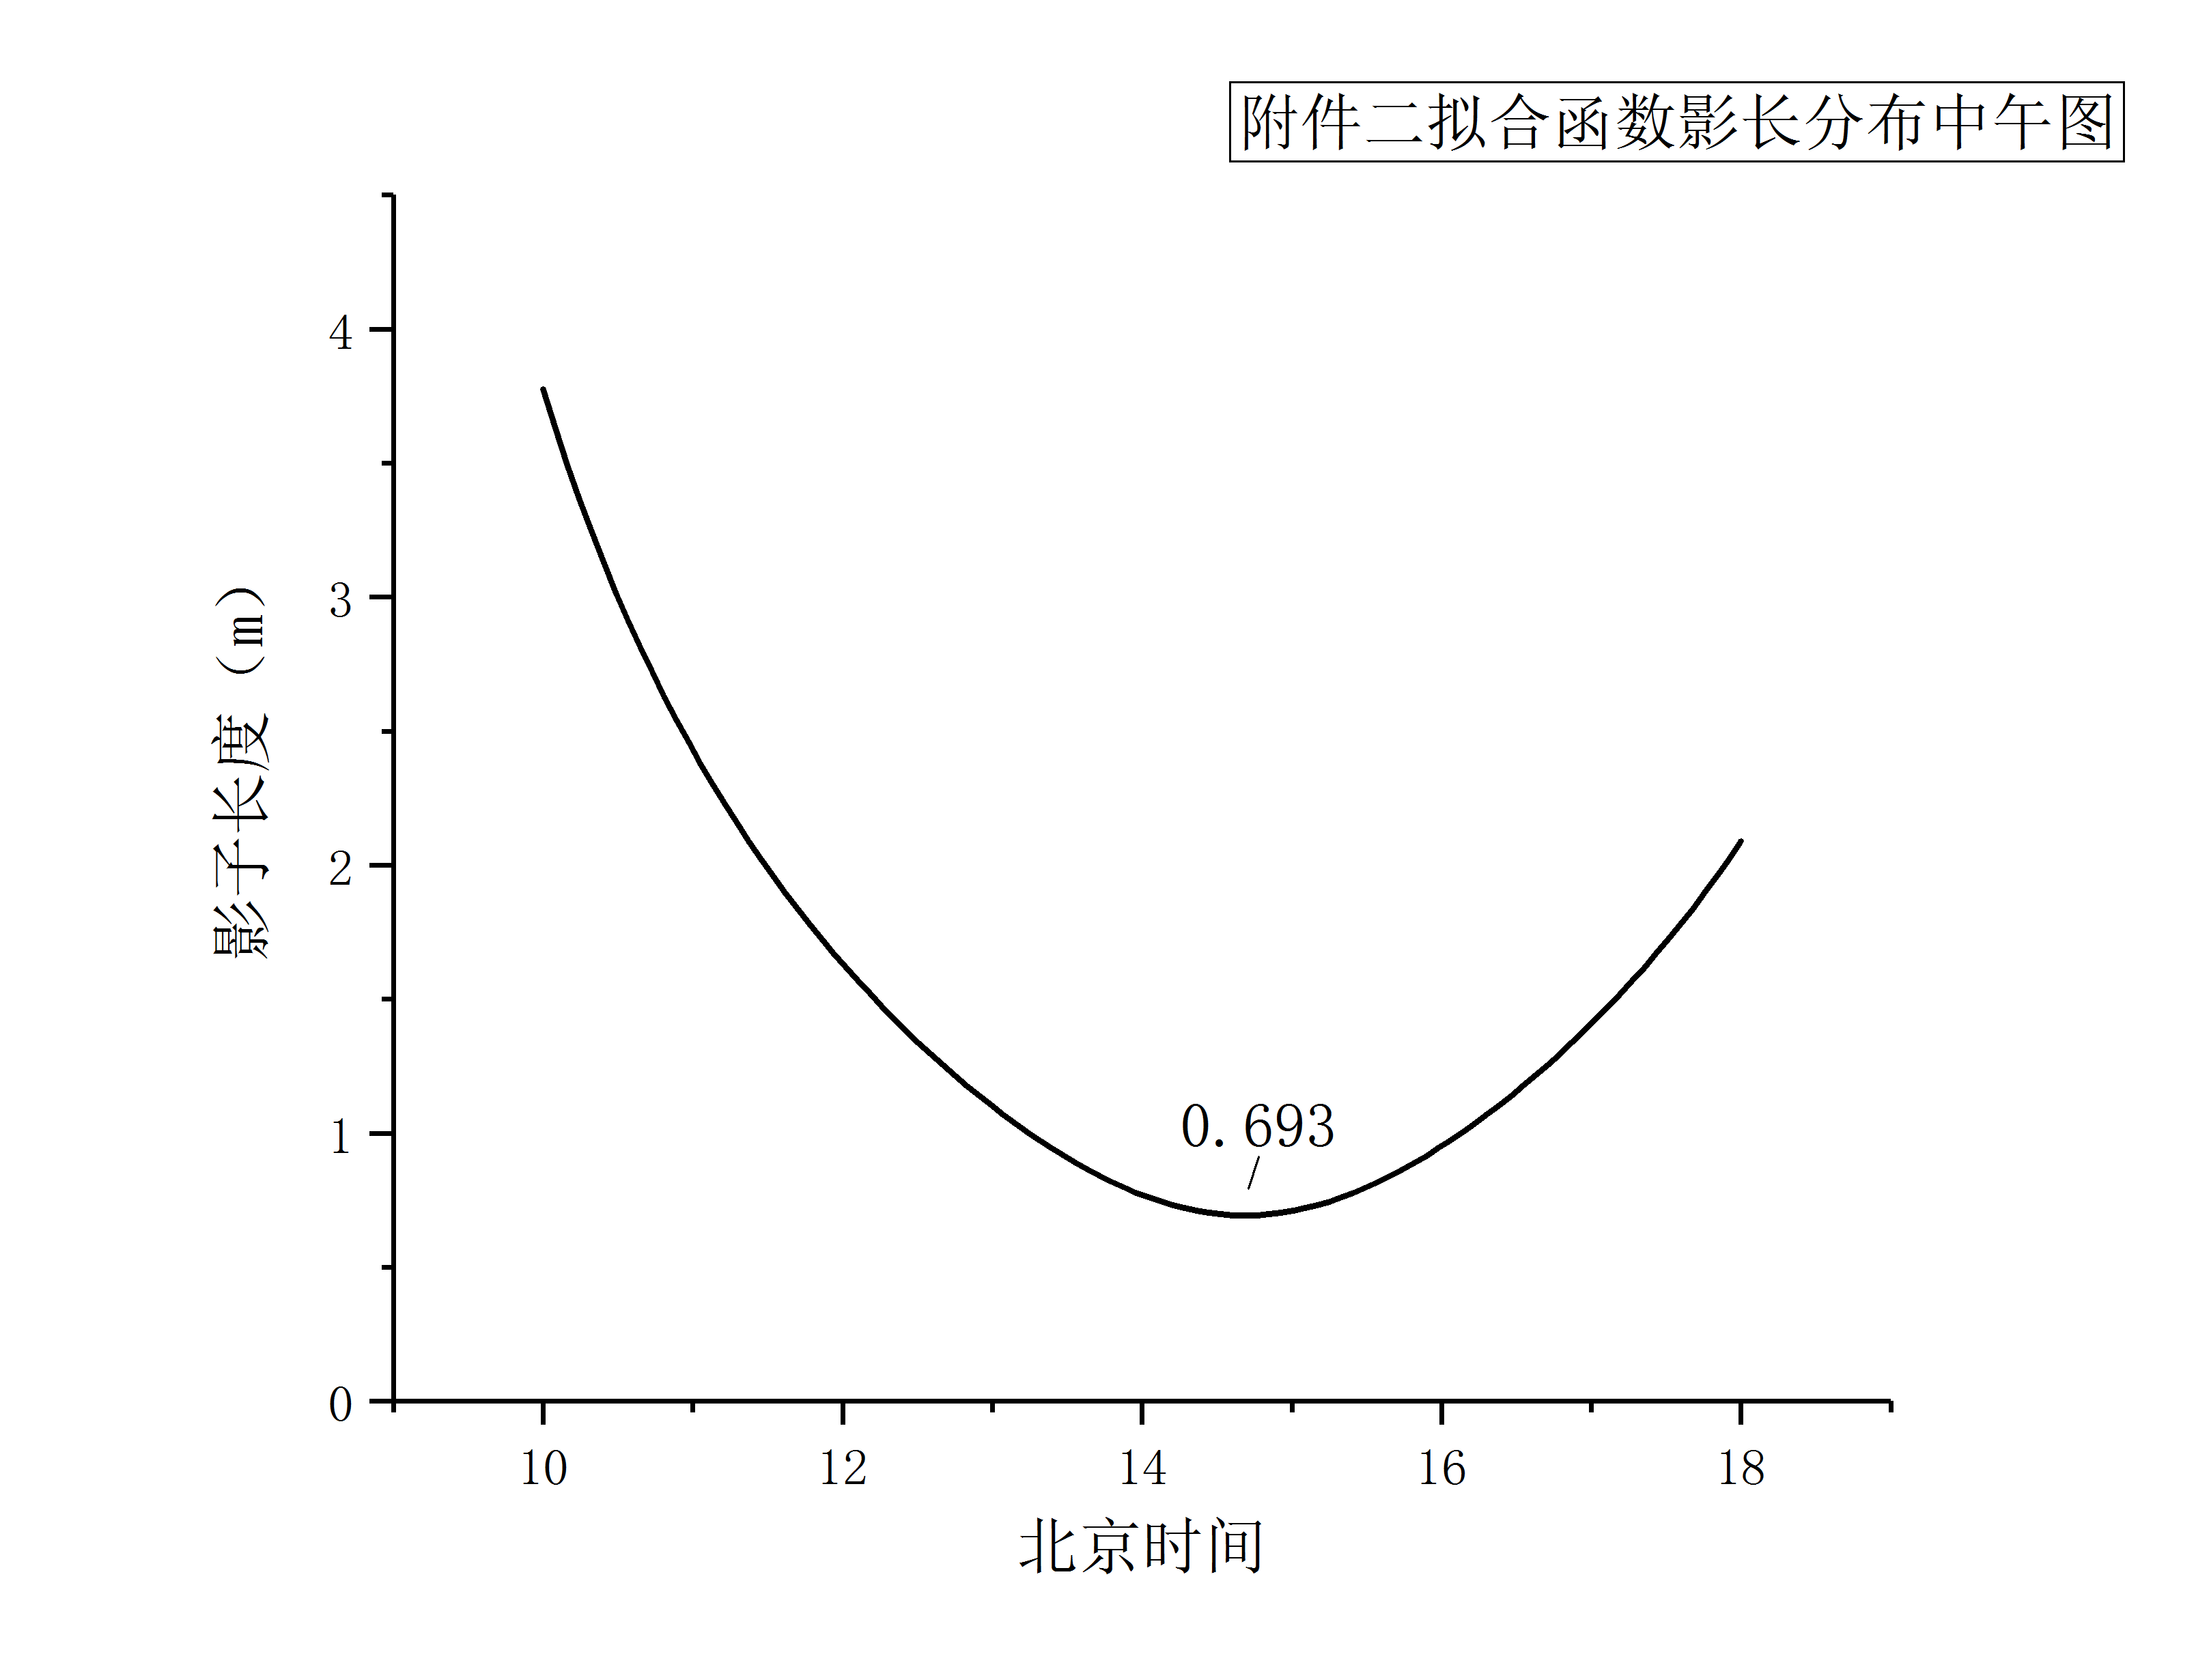
\includegraphics[width=.95\textwidth]{images/yanzheng3.png}
		\caption{拟合函数中午影长曲线图}
		\label{yanzheng3}
	\end{minipage}\hfill
	\begin{minipage}{.45\textwidth}
		\centering
		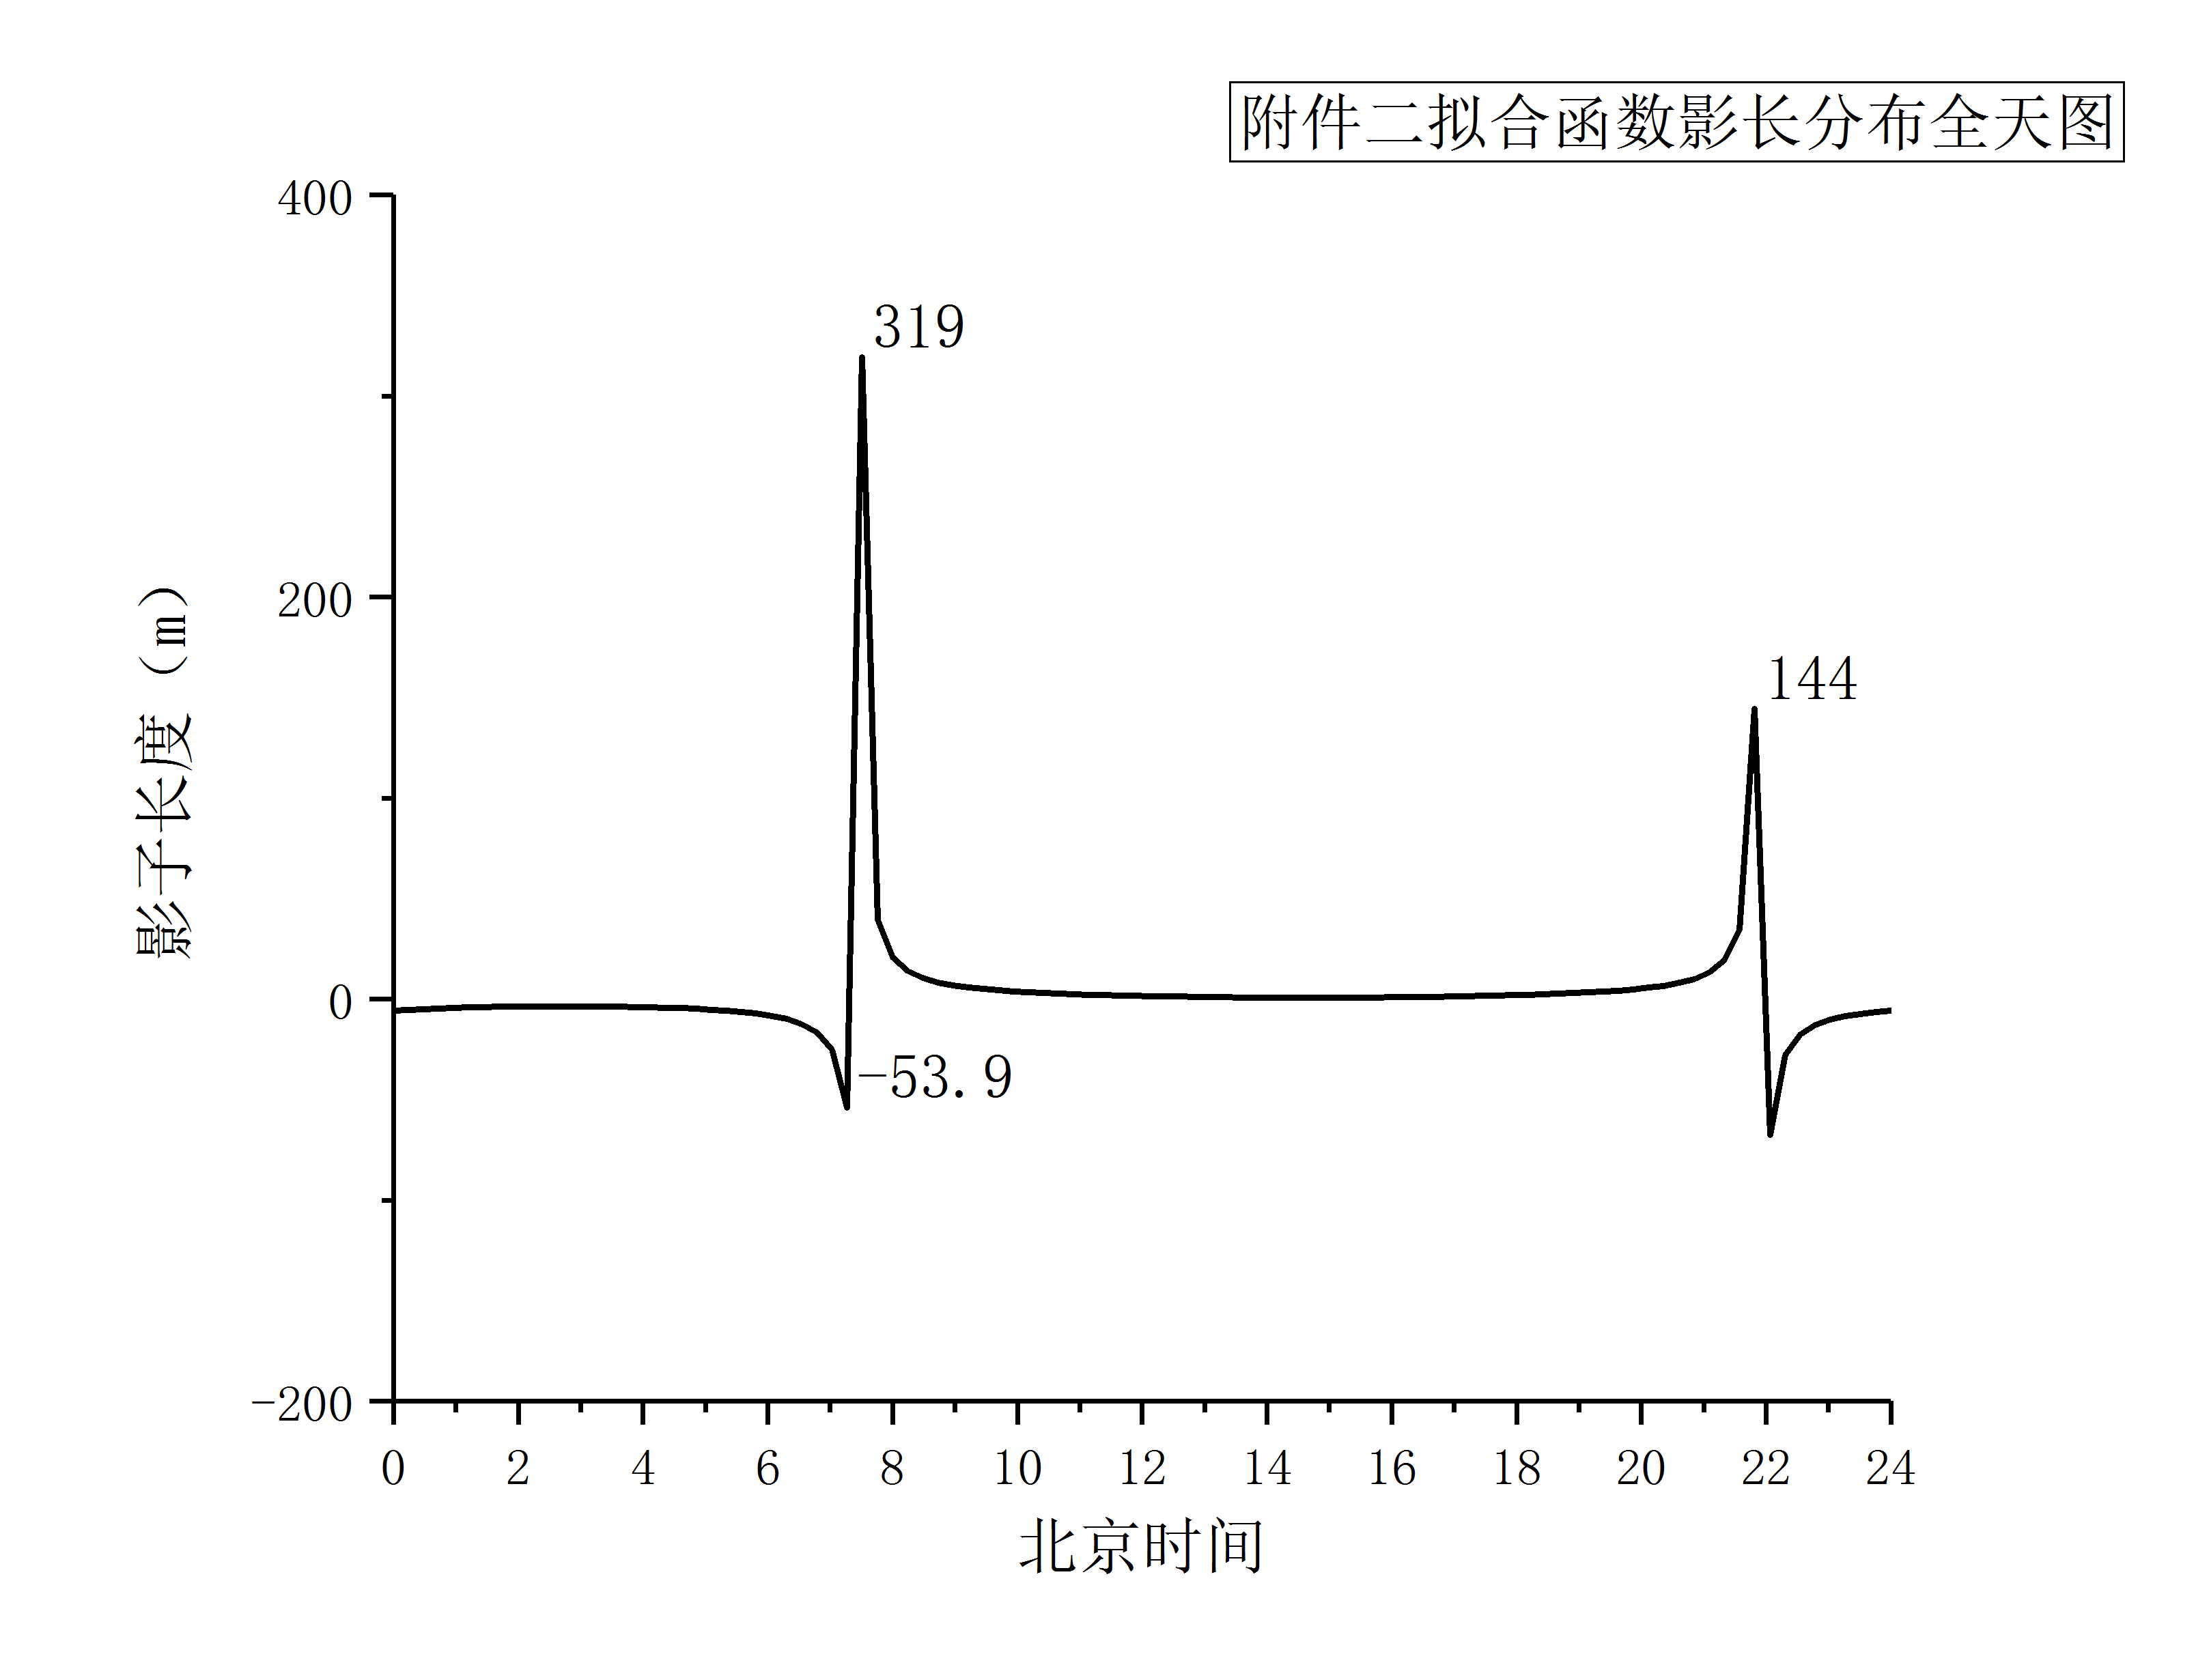
\includegraphics[width=.95\textwidth]{images/yanzheng4.png}
		\caption{拟合函数全天影长曲线图}
		\label{yanzheng4}
	\end{minipage}	
\end{figure}

进而发现所拟合的函数仍与问题一中函数高度相似,可以继续用于下面的变量预测:
$L=|A_1|=1.99099,\psi=arccos(A_2)=39.8433^\circ$,而$N=141.4411$。

我们同样采用遗传算法求解(三个变量),得到结果如表~\ref{answer2}~。

\begin{table}[H]
	\centering
	\caption{遗传算法所得结果}\label{answer2}
	\begin{tabular}{cccc}
		\toprule[1.5pt]
		纬度& 杆长&积日&适应度函数量级 \\
		\midrule[1pt]
		35.1382 &   1.6540 &  116.6 &-7\\
		33.9814 &  1.8642  &  231.3&-7\\
	---&   ---  & ---  &---\\
	39.5341  & 2.0403 & 203.3 & -7\\
	-37.8581  & 1.8939  &316.6  & -7\\
		--- &   ---   &  ---\\

		40.9046  & 1.8845 &151.8  & -7\\
		\bottomrule[1.5pt]
	\end{tabular}
\end{table}
由于此处遗传算法求出的较优解不是很集中,表格中仅筛选了满足适应度函数量级达到-7以上的较优解。可见纬度预测值$39.8433^\circ$、杆长预测值两米均十分可靠。而积日$N$虽然偏差较大,但也可以接受。注意到纬度基本对称分布,推测太阳直射点在赤道附近,选取积日为151.8的与231.3的解作为最可能日期。故而可以推测最可能处于新疆西部地区。时属4月份或七月份。




\subsubsubsection{附件三数据对应模型的求解与分析}
$\qquad$Origin拟合报告如表~\ref{baogao3}~。拟合效果较为乐观,$R^2=1$。在MATLAB中求出此函数在北京时间12.6504时达影长最小值3.4685米。从而计算得到经度$\phi=110.2440^\circ$。
\begin{table}[!htbp]
	\centering
	\caption{附件三函数拟合报告}\label{baogao3}
	\begin{tabular}{cc}
		\toprule[1.5pt]
		参数& 值 \\
		\midrule[1pt]
		A1	&$3.03565\pm 0.02534$\\
		A2	&$0.88044 \pm 0.0078$\\
		b1	&$3.31186\pm 4.32682\times 10^{-4}$\\
		b2  &$0.57619 \pm0.03194$\\
		b3  &$17.27732 \pm 34.97774$\\
		Reduced Chi-Sqr &$1.3983\times10^{-9}$\\
		R平方(COD)&	1\\
		\bottomrule[1.5pt]
	\end{tabular}
\end{table}
同样为了确保在此拟合下是否仍能准确预测杆长、纬度、甚至积日,我们画出拟合出的函数影子长度变化曲线如图\ref{yanzheng5}、\ref{yanzheng6}与问题一中的图\ref{yanzheng2}、\ref{yanzheng1}进行对比。进而发现所拟合的函数仍与问题一中函数高度相似,可以继续用于下面的变量预测:
$L=|A_1|=3.03565,\psi=arccos(A_2)= 28.3045^\circ$,而$N=354.66$。

\begin{figure}[H]
	\centering
	\begin{minipage}{.45\textwidth}
		\centering
		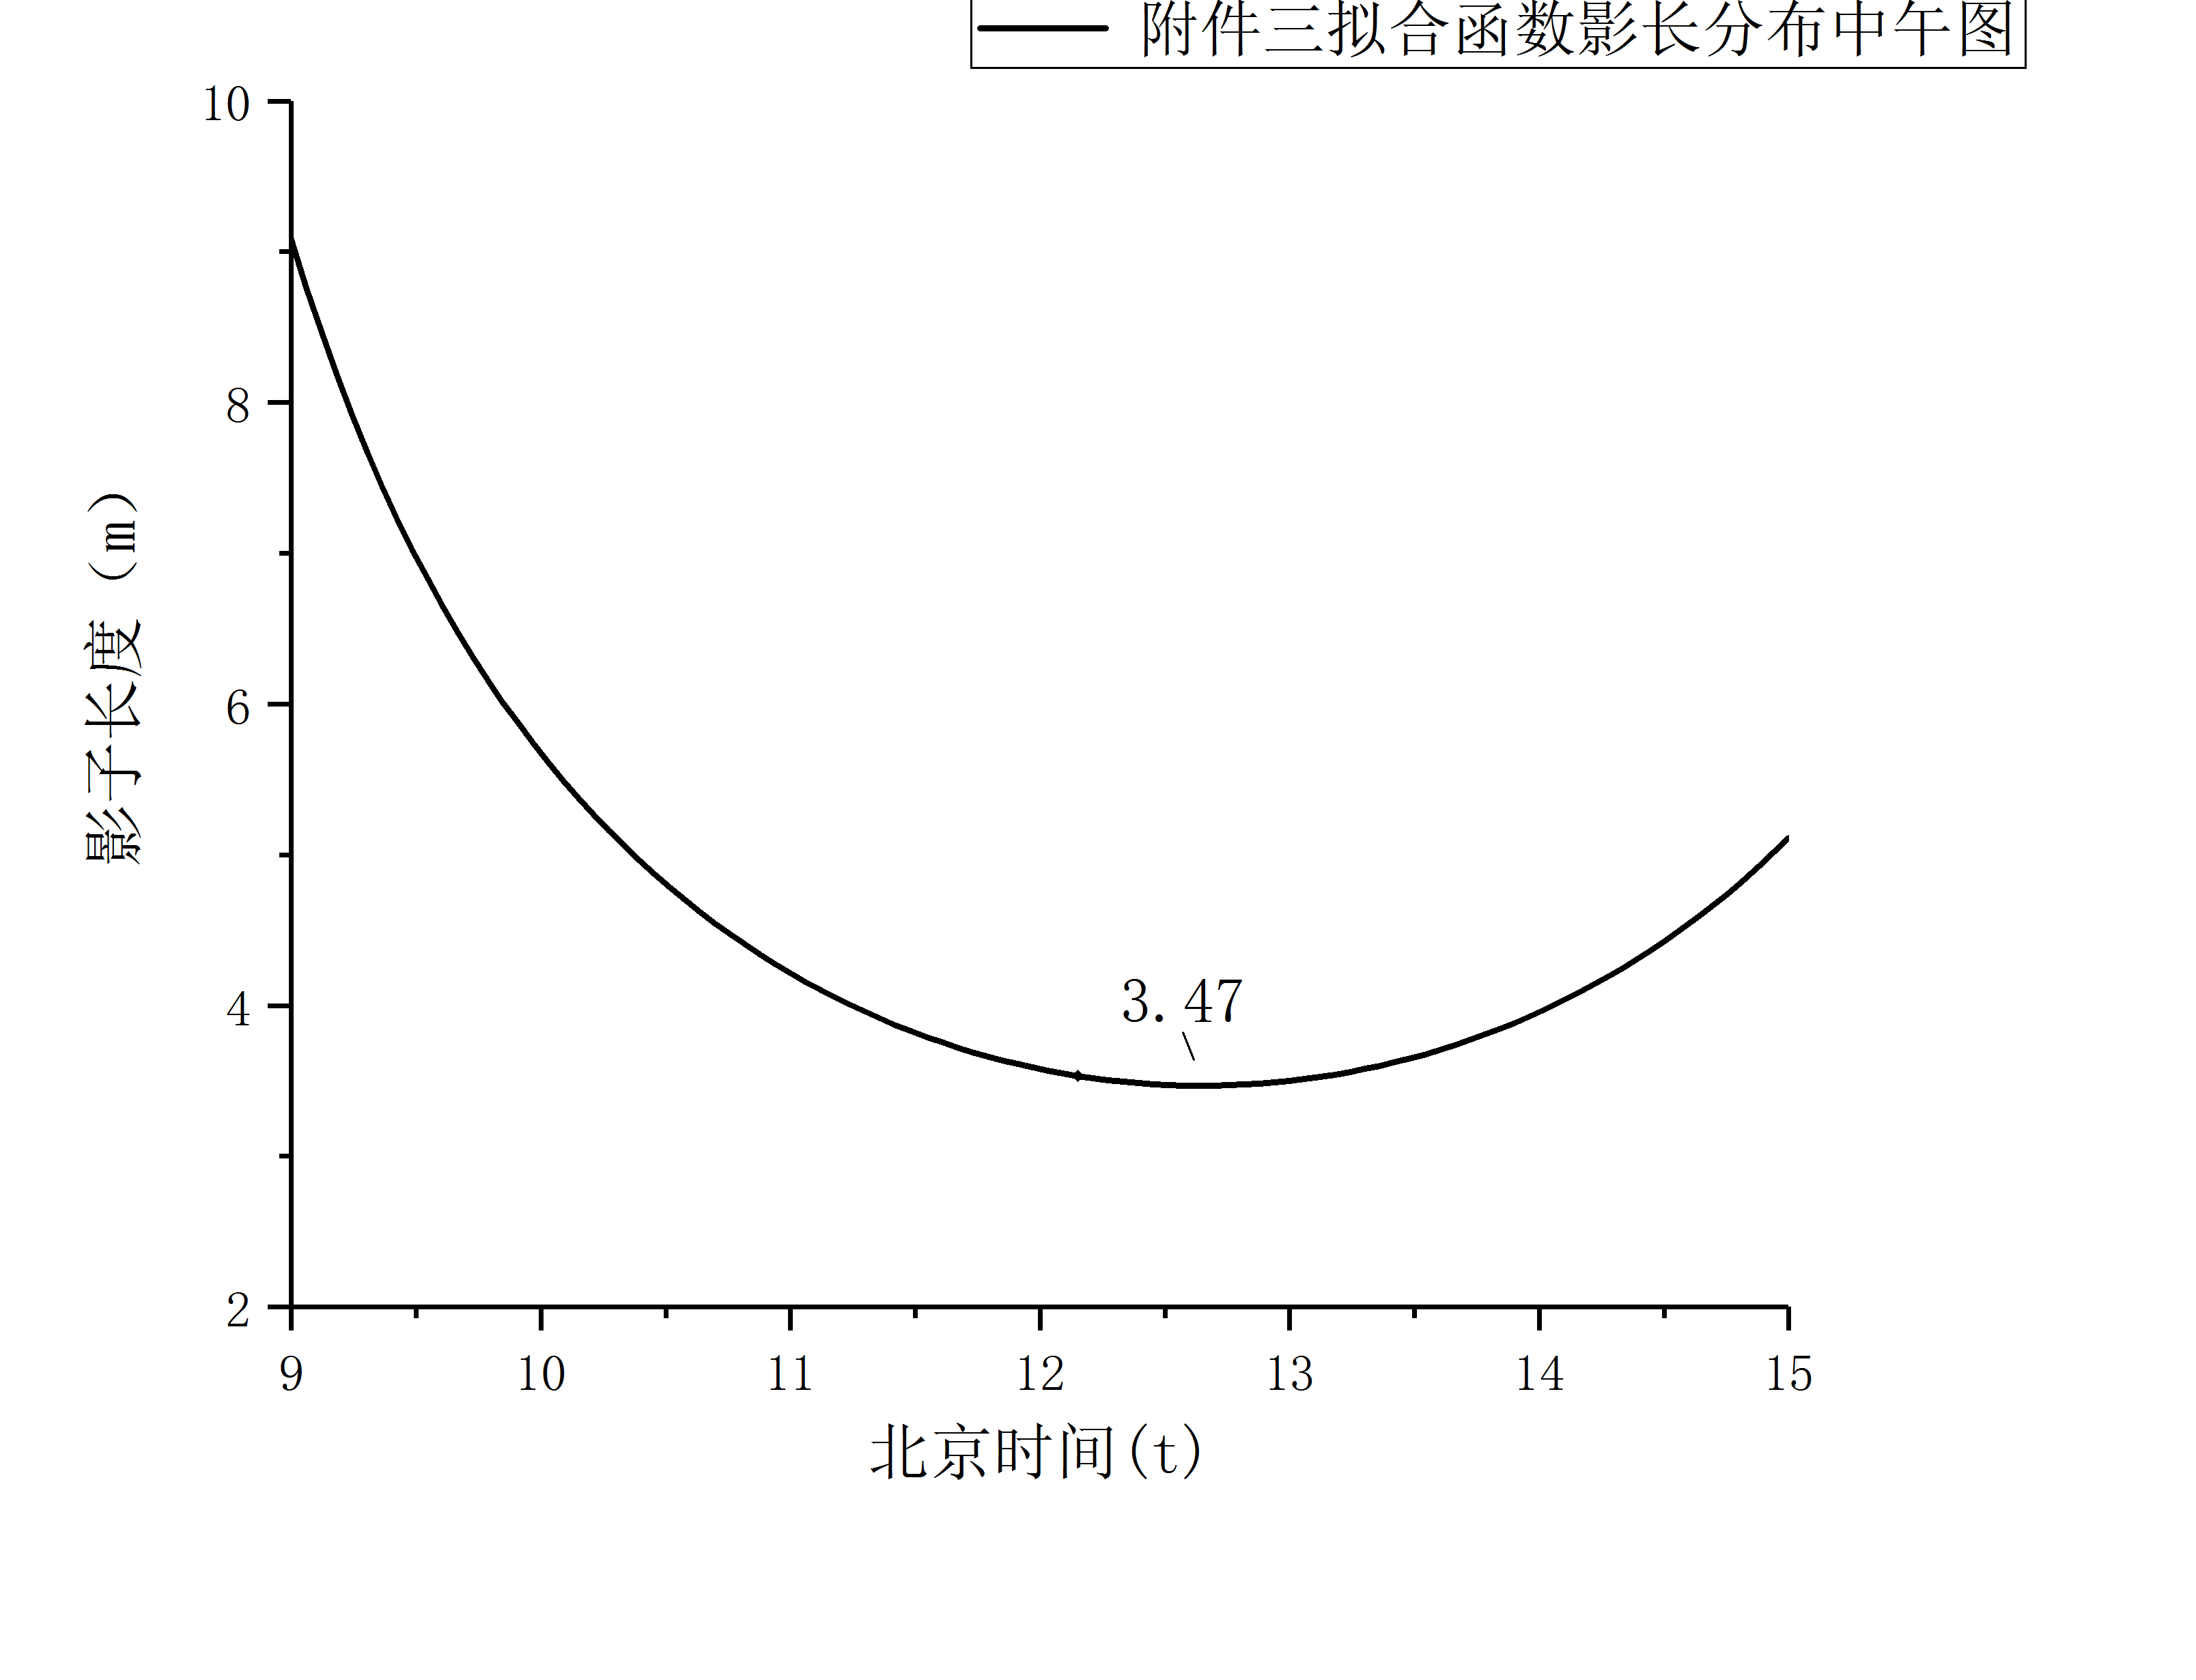
\includegraphics[width=.95\textwidth]{images/yanzheng5.png}
		\caption{拟合函数中午影长曲线图}
		\label{yanzheng5}
	\end{minipage}\hfill
	\begin{minipage}{.45\textwidth}
		\centering
		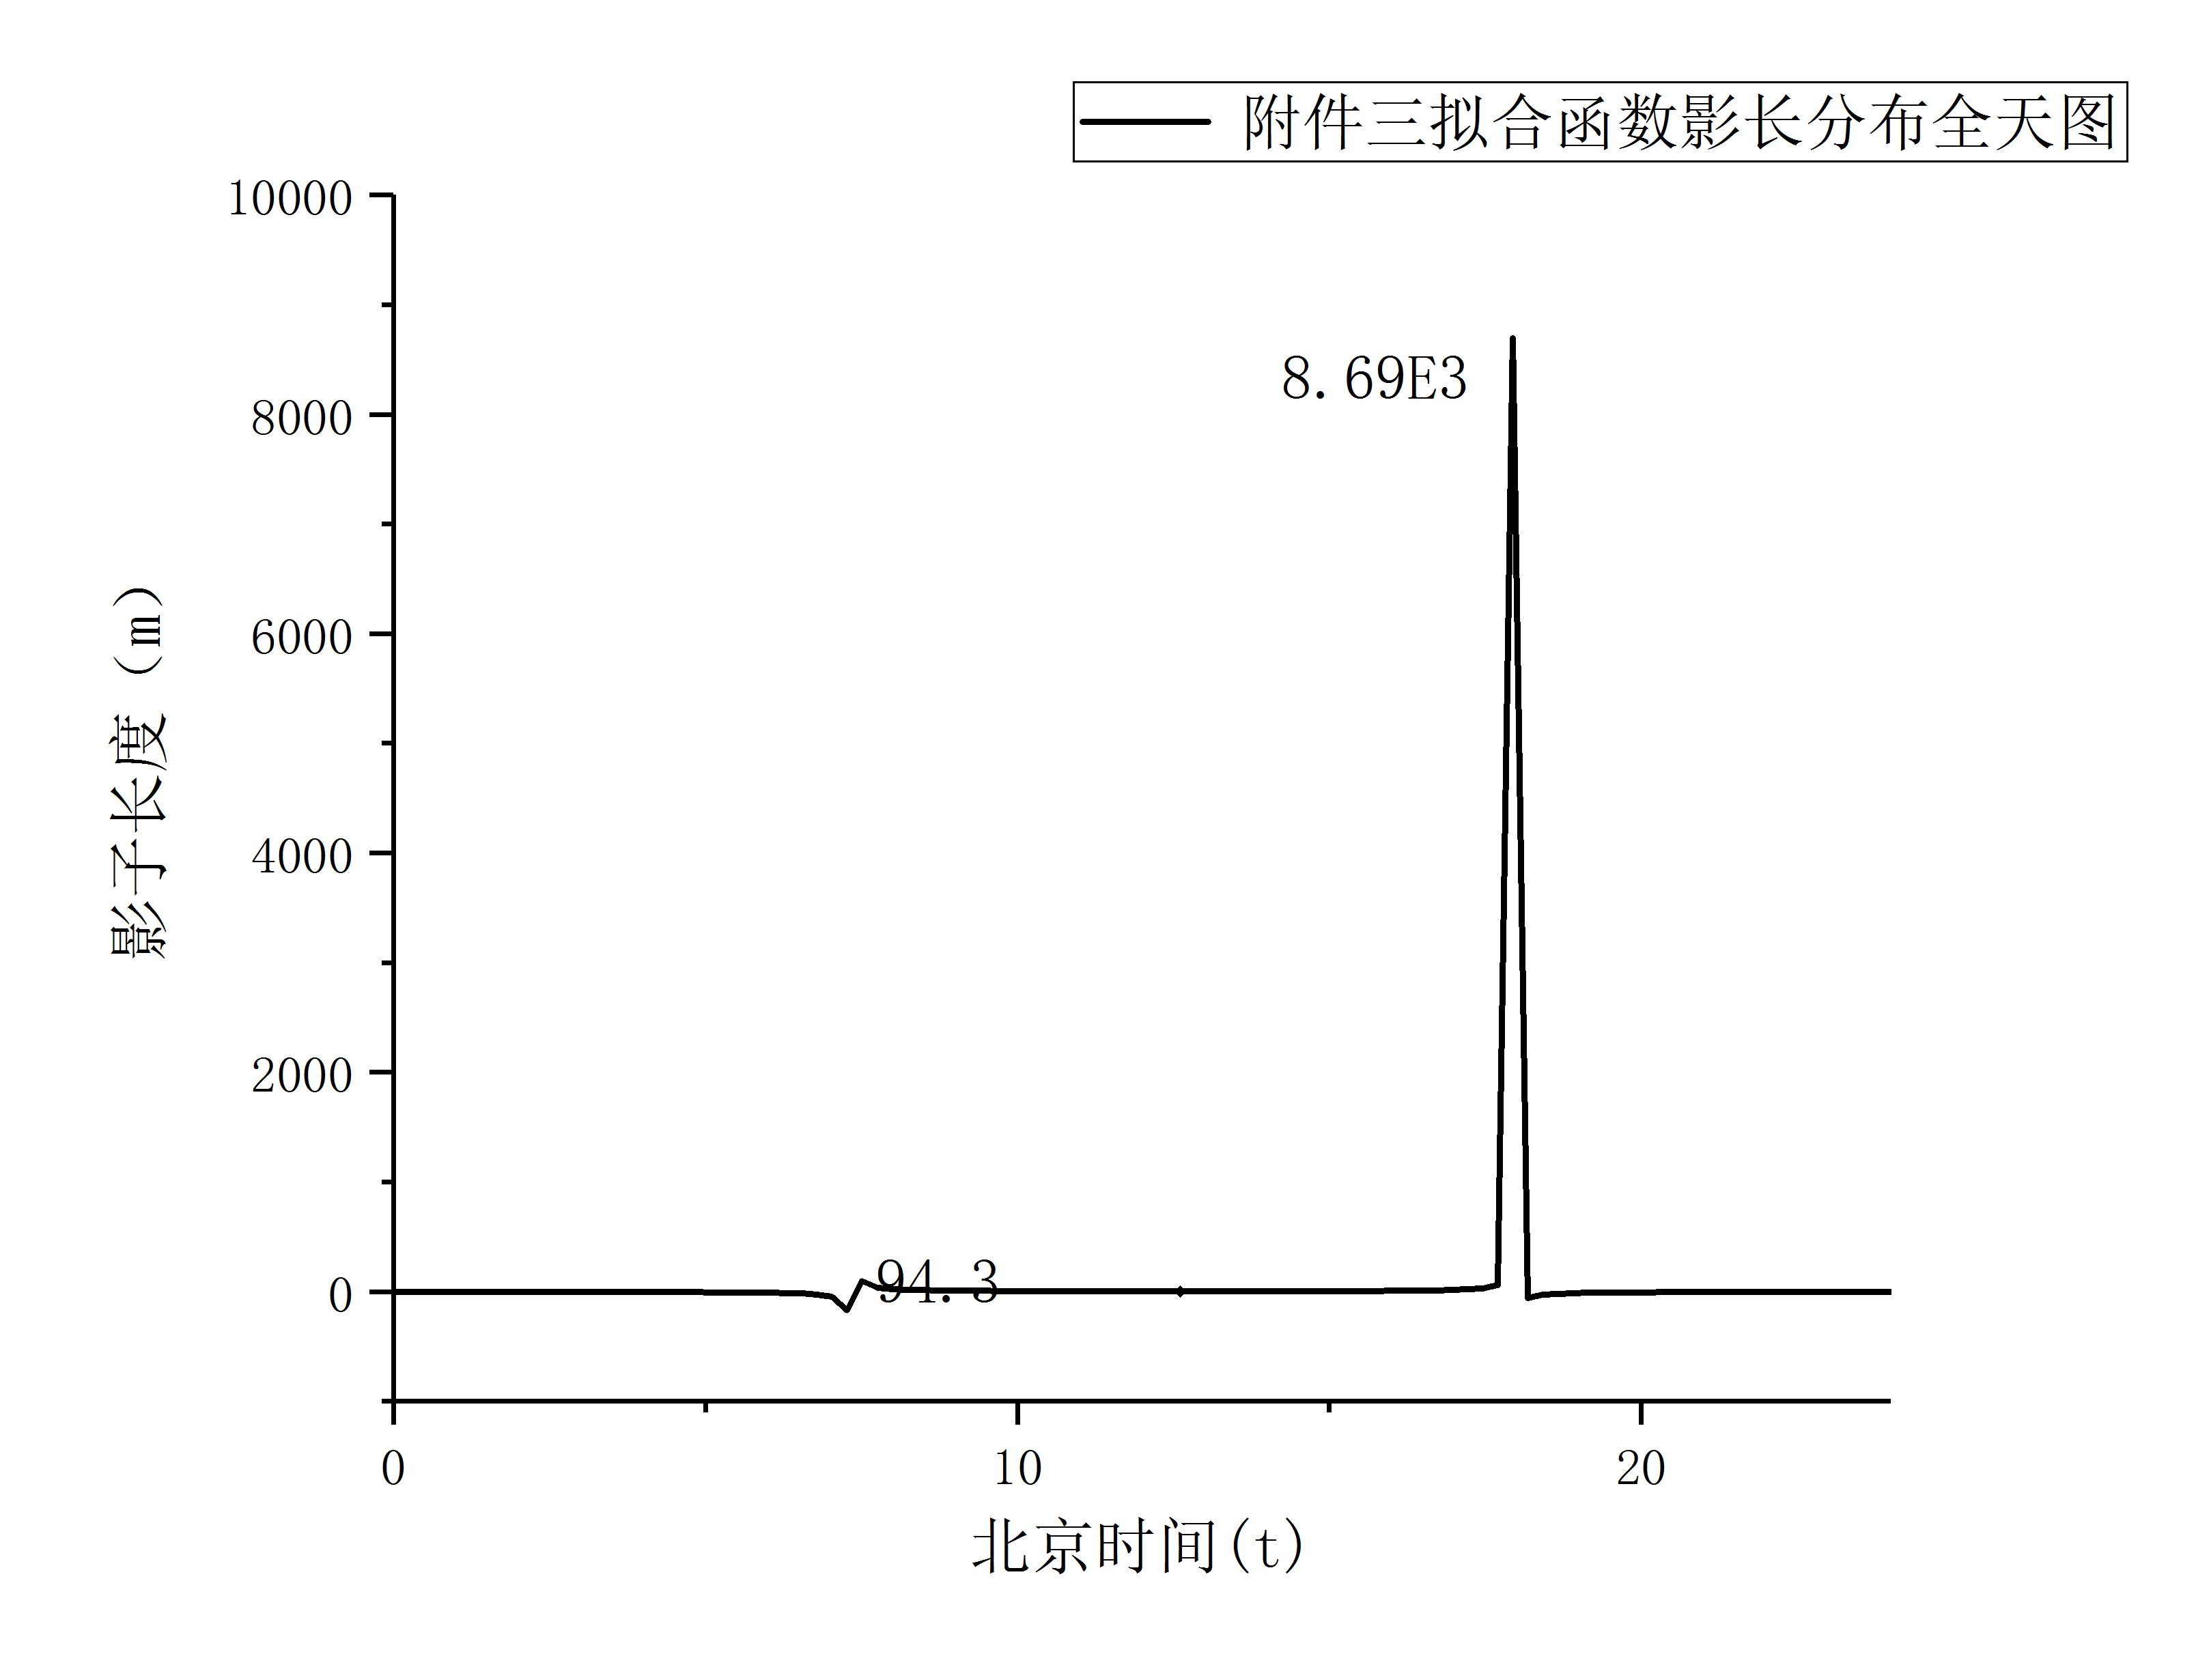
\includegraphics[width=.95\textwidth]{images/yanzheng6.png}
		\caption{拟合函数全天影长曲线图}
		\label{yanzheng6}
	\end{minipage}	
\end{figure}

本文同样采用遗传算法求解(三个变量),最终可以得到如下结果:纬度主要分布在$[29.44,29.85]$与$[50.87,54.72]$之间;杆长主要分布在$[1.06,1.35]$与$[3.14,3.51]$之间;而积日则主要分布在$[305.9,329.2]$之间。亦即纬度与杆长预测较为准确,而积日的预测值偏小。原因可能有二,一是附件所给数据存在误差,二是遗传算法过早陷入了局部最优解。综合来说二的可能性更大,故而可以推测:最可能位于湖南张家界地区,时属10月份。


\subsection{问题四基于图像处理的反演模型的建立与求解}
本问题由于相机位于杆的前方,影子的成像实际为真实影子的中心投影,图像中直接测量得影子长度并非真实影子长度,需要利用透视变换将图像转换为光线垂直于地面的正投影来计算影子长度。
\subsubsection{模型的准备}
\subsubsubsection{透视变换}
$\qquad$透视变换(Perspective Transformation)是指利用透视中心、像点、目标点三点共线的条件,按透视旋转定律使承影面(透视面)绕迹线(透视轴)旋转某一角度,破坏原有的投影光线束,仍能保持承影面上投影几何图形不变的变换。其本质是将图像投影到一个新的视平面,由资料 中可知通用变换公式为

\begin{equation}
[x^{'},y^{'},w^{'}]=[u,v,w]\times T
\end{equation}
\begin{equation}
\left\{ \begin{array}{l}
x = \frac{{x^{'}}}{{w^{'}}}\\
y = \frac{{y^{'}}}{{w^{'}}}
\end{array} \right.
\end{equation}

其中,$(u,v)$为原始图像的像素坐标,$(x,y)$为变换后图像的像素坐标,$T$为透视变换矩阵
\begin{equation}
\left[ \begin{array}{l}
{a_{11}},{a_{12}},{a_{13}}\\
{a_{21}},{a_{22}},{a_{23}}\\
{a_{31}},{a_{32}},{a_{33}}
\end{array} \right]
\end{equation}
经过计算,透视变换的数学表达为:
\begin{equation}
\begin{array}{l}
x = \frac{{{x^{'}}}}{{{w^{'}}}} = \frac{{{a_{11}}u + {a_{21}}v + {a_{31}}}}{{{a_{13}}u + {a_{23}}v + {a_{33}}}}\\
y = \frac{{{y^{'}}}}{{{w^{'}}}} = \frac{{{a_{12}}u + {a_{22}}v + {a_{32}}}}{{{a_{13}}u + {a_{23}}v + {a_{33}}}}  \label{bianhuan}
\end{array}
\end{equation}
所以,对于给定的变换前后的4组对应图像像素坐标,即可求出上式中的各个参数。
\subsubsubsection{视频与图像处理}
$\qquad$按以下步骤进行操作:
\begin{enumerate}
	\item 将视频载入matlab,每隔一分钟取一帧,共得到41张图片。
	\item 调用opencv图像处理函数库编写程序,载入所有图片,对图片进行透视变换,变换前取点如图\ref{toushi}所示(假设真实世界中$AB,CD$两条直线相互平行)。
	 \begin{figure}[H]
		\centering
		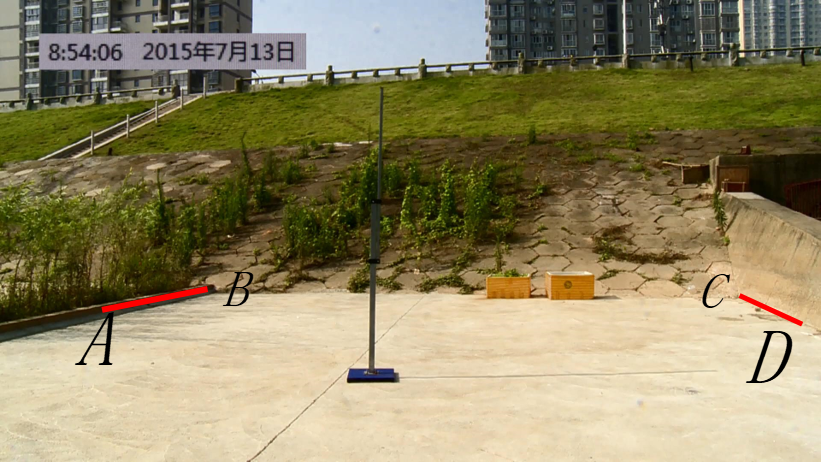
\includegraphics[scale=0.4]{images/toushi.png}
		\caption{变换前取点}
		\label{toushi}
	\end{figure}   
	原图像选取的点依次为$A(274,738),B(508,683),C(1727,683),D(1871,738)$。变换后点依次为$A^{'}(1,368),B^{'}(1,1),C^{'}(1000,1),D^{'}(1000,368)$。
	
	\item 参考资料对变换后的图像进行预处理如图\ref{chuli}
	 \begin{figure}[H]
		\centering
		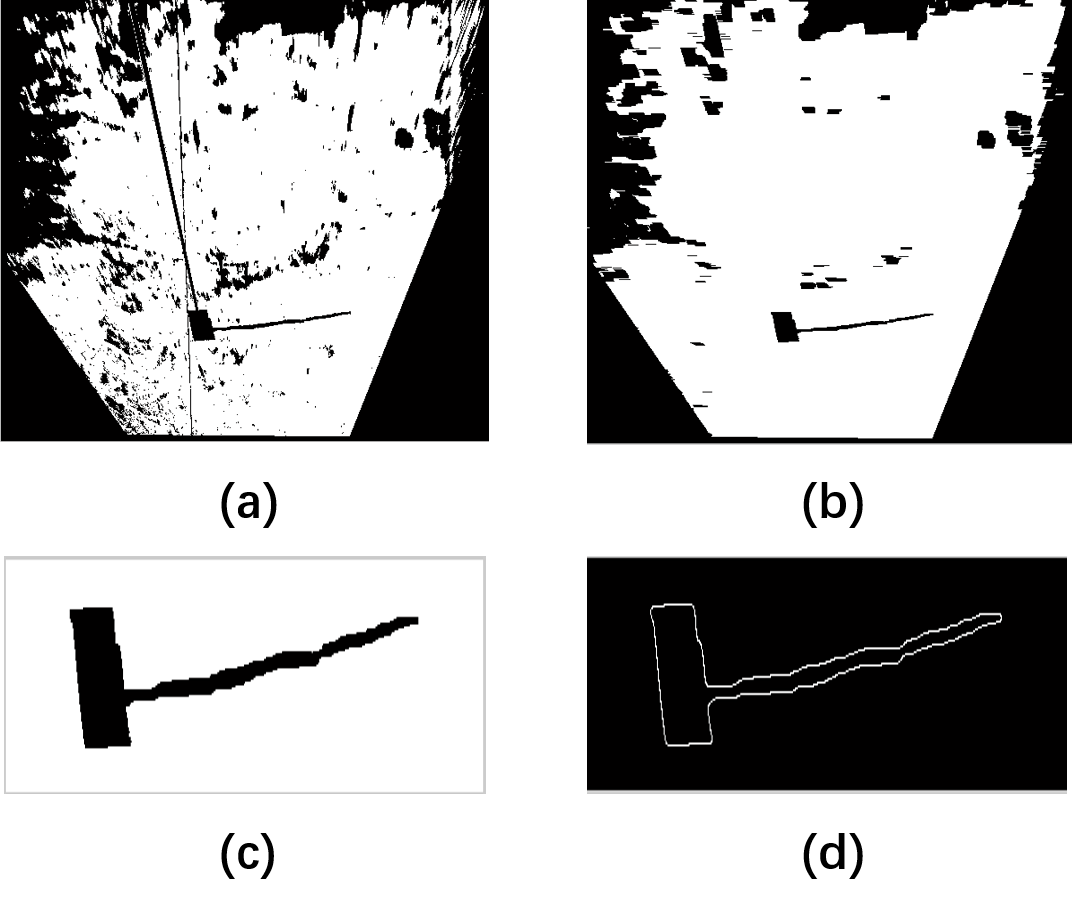
\includegraphics[scale=0.4]{images/chuli.png}
		\caption{变换后的处理}
		\label{chuli}
	\end{figure} 
   \begin{enumerate}
   	\item 对图像进行灰度化,二值化
   	\item 以线性结构元素对图像进行闭运算,填充图像空洞
   	\item 截取影子部分
   	\item 对截取后的图像中所有连通区域进行标号,仅保留联通区域面积最大的部分(即影子部分),利用canny算子进行边缘检测
   \end{enumerate}

\end{enumerate}
\subsubsection{计算影子长度模型的建立}	
通过计算得出,变换矩阵
\begin{equation}
T = \left[ {\begin{array}{*{20}{c}}
	{ - 0.0867}&0&0\\
	{ - 0.3703}&{ - 0.9261}&{ - 0.0015}\\
	{296.8916}&{632.4676}&1
	\end{array}} \right]
\end{equation}
发现其中$a_{12}=0,a_{13}=0$,结合公式\ref{bianhuan}可知,变换后的$y$只和变换前的$v$有关,即如果变换前若干点的像素纵坐标相同,变换后的像素纵坐标也相同。所以考虑在图像的水平方向上添加辅助线来计算影长的实际距离。

对于截取的初始图像中,假设以杆与地面的交点像素坐标$O(x_0,y_0)$,杆的真实长度为$Z$,杆的顶端像素坐标$(x_1,y_1)$,这里近似认为$x_0=x_1$。即杆为严格垂直于地面的。此时杆在图片中的长度
\begin{equation}
Z^*=|y_0-y_1|
\end{equation}
以$O$为顶点,沿图像$x$轴正方向做辅助线,真实长度为$K=0.5\times Z $,在初始图像长度上为$K^*=0.5\times Z^*$,参见图~\ref{tuyi}~。对于变换后的图像,由上述理论,并结合图~\ref{tuer}~,在此时的视平面中,影子在图片中的长$S^*$ 与影子的真实长度$S$有以下关系
\begin{equation}
\frac{{{K^{**}}}}{K} = \frac{{{S^*}}}{S}
\end{equation}
\begin{figure}[h]
	\centering
	\begin{minipage}{.45\textwidth}
		\centering
		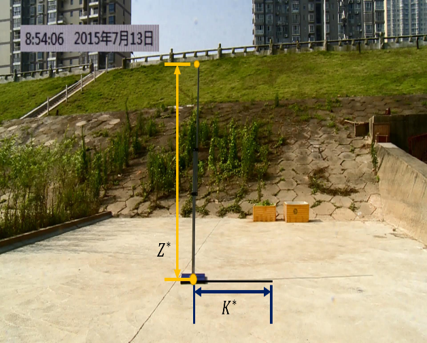
\includegraphics[width=.95\textwidth]{images/tuyi.png}
		\caption{透视变换前}
		\label{tuyi}
	\end{minipage}\hfill
	\begin{minipage}{.45\textwidth}
		\centering
		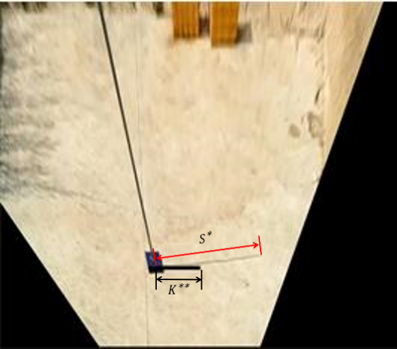
\includegraphics[width=.95\textwidth]{images/tuer.png}
		\caption{透视变换后}
		\label{tuer}
	\end{minipage}	
\end{figure}

其中,$K^{**}$为辅助线在变换后图片中的长度。对于$S^{*}$的计算,在上述对初始图像进行处理后,得到影子的白色轮廓,灰度值为1,对图片矩阵由右向左进行逐个监测,检测到白色轮廓时记下此时像素点坐标$(x_1^*,y_1^*)$,假设给定处理后图片上的杆与地面交点像素坐标$(x_0^*,y_0^*)$,则:
\begin{equation}
{S^*} = \sqrt {{{(x_1^* - x_0^*)}^2} + {{(y_1^* - y_0^*)}^2}} 
\end{equation}
\subsubsection{直杆地点反演模型的求解与分析}
对截取的所有41张图片利用上述模型求解影子的实际长度。部分结果如表~\ref{baogao4}~所示。不过经尝试发现,由于这次拟合所用的数据是自己经过图像识别采集的,并不符合问题一中的函数结构,因此拟合效果非常差,即便是用来求经度,也十分的不合理。最终我们采用了二次拟合的方法计算出经度为$111^\circ$。
\begin{table}[!htbp]
	\centering
	\caption{图像处理所得影子长度}\label{baogao4}
	\begin{tabular}{cc}
		\toprule[1.5pt]
		北京时间($t$)& 影子长度($m$) \\
		\midrule[1pt]
		8.90 &	2.61 \\
		8.92 &	2.59 \\
		8.93 &	2.58 \\
		-- &	-- \\
		9.50 &	2.01 \\
		9.52 &	2.00 \\
		9.53 &	1.99 \\
		9.55 &	1.98 \\
		9.57 &	1.97 \\
		\bottomrule[1.5pt]
	\end{tabular}
\end{table}
\subsubsubsection{拍摄日期已知(7月13日)}	
$\qquad$此问题化归成了问题二。采用遗传算法求得纬度基本都为$24.88^\circ$。故而推测地点在广西桂林。



\subsubsubsection{拍摄日期未知}	
$\qquad$如若拍摄日期也未知实际上便是问题三的求解。采用同样的算法可得如表~\ref{answer2}~所示结果。
\begin{table}[H]
	\centering
	\caption{遗传算法所得结果}\label{answer2}
	\begin{tabular}{ccc}
		\toprule[1.5pt]
		纬度&积日&可能地点 \\
		\midrule[1pt]
	35.6709&	201	&陕西渭南市\\
	39.7608&	198	&内蒙古鄂尔多斯市\\
	-35.365&	13	&-\\
	36.9887	&129&	陕西榆林市\\
	-28.3574&	291	&-\\
	-35.3651&	13&	-\\
	-32.7052&	295&	-\\
	35.4806	&201	&陕西渭南市\\
	34.0168	&126	&陕西省商洛市\\
	34.1508&	126&	陕西省商洛市\\
	-35.392	&12&	-\\
		\bottomrule[1.5pt]
	\end{tabular}
\end{table}
故而可以推测最优可能位于陕西省商洛、渭阳一带。日期可能处于一月初或者六七月份。

\subsubsection{问题四的灵敏度分析}
本问题中的经度最终由二次函数拟合,所以在经度的计算上存在一定误差。表\ref{answer2}给出了有日期时和无日期时经度变化对求解结果的影响。

\begin{table}[H]
	\centering
	\caption{有拍摄日期}\label{answer2}
	\begin{tabular}{ccc}
		\toprule[1.5pt]
经度变化值	&纬度变化值&	纬度变化率\\
		\midrule[1pt]

-2	&34.8067&	39.89\%\\
-1&	38.799	&55.94\%\\
0&	24.8808	&0.00\%\\
1&	18.0161	&-27.59\%\\
2&	14.4676	&-41.85\%\\

		\bottomrule[1.5pt]
	\end{tabular}
\end{table}
由表\ref{answer2}可以看出,在有日期时,对由我们拟合出的一天中影长随时间变化曲线来说,计算得出的经度发生微小的变化就会很大程度上影响最终的地理位置,说明拍摄地地理位置受经度变化影响较为灵敏,因此需要改进经度计算方法,提高经度的准确性;

\begin{table}[H]
	\centering
	\caption{无拍摄日期}\label{answer3}
	\begin{tabular}{ccccc}
		\toprule[1.5pt]
经度变化值&	纬度变化值&	积日变化值&	纬度变化率&	日期变化率\\
		\midrule[1pt]

-2	&35.3693&	186&	-4.38\%	&44.19\% \\
-1&	36.318&	132	&-1.81\%&	2.33\%\\
0&	36.9887	&129&	0.00\%&	0.00\%  \\
1&	38.2441&	124	&3.39\%	&-3.88\%\\
2&	33.7315	&221&	-8.81\%	&71.32\% \\
		\bottomrule[1.5pt]
	\end{tabular}
\end{table}
由表\ref{answer3}可以看出,在日期未知的情况下,经度在一定范围内变化时,纬度变化率非常小,说明纬度受经度变化影响较小,而日期的变化在初始计算出的经度基础上小范围($\pm 1$度)内变化时,变化率也非常小,而在较大范围($\pm 2$度)内变化时,变化率很大,说明日期未知时,纬度受经度变化影响较小,日期在一定程度上受经度变化影响较小。综上所述,为了更加准确的确定视频拍摄地的地点与日期,在计算经度的过程中需要不断改进与完善模型,使计算得出的经度更加准确,从而减小误差,使结果更加精确。




\newpage

\section{模型的评价}
\subsection{模型的优点}
\begin{enumerate}
  \item  在问题一中考虑了真太阳时,对平太阳时进行了修正。
  \item 拟合采用依据问题一函数结构自定义的拟合函数,高度近似了原影长函数并可以给出准确的预测值。
  \item  问题四中图像处理能够减少透视投影引起的影子长度的误差。
\end{enumerate}

\subsection{模型的缺点}
\begin{enumerate}
  \item 对图像的透视变换及一系列的处理过程中会在一定程度上对图像造成失真,导致测量结果不准确.
  \item 问题四中的二次拟合会造成一定误差.
  \item 利用遗传算法得出的解可能为局部最优解,与真实解存在一定差距。
\end{enumerate}



\subsection{模型的推广}
本文中的基于函数结构的自定义非线性拟合可以推广到很多种实际问题中,不仅可以拟合参数,也可以提供预测\cite{abc}。\cite{t-SNE} \cite{scikit-learn,CC01a} \cite{kingma2013auto}






\makebox{}










\bibliographystyle{plain}%%%参考文献的条目的编号是按照引用的顺序, 而不是按照作者的字母顺序
\bibliography{citation}

%\begin{thebibliography}{5}
%	\bibitem{1} 张志鹏,崔克楠,李厚彪. 太阳影子定位的时空分析[J]. 实验科学与技术,2017,15(01):39-42+49. [2017-08-29].
	
%    \bibitem{2} 周诗豪. 直杆太阳影子变化长度的建模分析[J]. 科技展望,2016,26(12):182. [2017-08-29].
    
%    \bibitem{3}  胡明晓.正交回归和一般最小二乘回归的几何误差分析[J]. 数理统计与管理,2010,29(02):248-253. [2017-08-29]. DOI:10.13860/j.cnki.sltj.2010.02.005
    
    
  %  \bibitem{4}  http://www.cnblogs.com/liekkas0626/p/5262942.html
    
 %  \bibitem{5}   精通MATLAB图像处理(第2版)   张强,王正林 编著  电子工业出版社 2012年4月1日 
   
%\end{thebibliography}

\newpage

\appendix
\section{附录}
\subsection{问题一源程序}



代码描述:\textbf{\textcolor[rgb]{0.98,0.00,0.00}{Input matlab source:}}
\lstinputlisting[language=Matlab,morekeywords={ones,intersect}]{./code/Find_path.m}

\subsection{问题二源程序}

代码描述: \textcolor[rgb]{0.98,0.00,0.00}{\textbf{Input C++ source:}}
\lstinputlisting[language=C++, morekeywords={alignas,continute,friend,register,true,alignof,decltype,goto,
	reinterpret_cast,try,asm,defult,if,return,typedef,auto,delete,inline,short,
	typeid,bool,do,int,signed,typename,break,double,long,sizeof,union,case,
	dynamic_cast,mutable,static,unsigned,catch,else,namespace,static_assert,using,
	char,enum,new,static_cast,virtual,char16_t,char32_t,explict,noexcept,struct,
	void,export,nullptr,switch,volatile,class,extern,operator,template,wchar_t,
	const,false,private,this,while,constexpr,float,protected,thread_local,
	const_cast,for,public,throw,std}]{./code/mcmthesis-sudoku.cpp}


代码描述: \textbf{\textcolor[rgb]{0.98,0.00,0.00}{Input matlab source:}}
\lstinputlisting[language=Matlab,morekeywords={ones,intersect}]{./code/nuclear_density.m}

\subsection{问题三源程序}

代码描述: \textcolor[rgb]{0.98,0.00,0.00}{\textbf{Input Python source:}}
\lstinputlisting[language=Python,morekeywords={plt,fig,ax}]{./code/t-SNE.py}

\subsection{问题四源程序}

代码描述: \textcolor[rgb]{0.98,0.00,0.00}{\textbf{Input R source:}}
\lstinputlisting[language=R]{./code/t-sne.R}


\end{document}
